\documentclass[twoside]{book}

% Packages required by doxygen
\usepackage{fixltx2e}
\usepackage{calc}
\usepackage{doxygen}
\usepackage[export]{adjustbox} % also loads graphicx
\usepackage{graphicx}
\usepackage[utf8]{inputenc}
\usepackage{makeidx}
\usepackage{multicol}
\usepackage{multirow}
\PassOptionsToPackage{warn}{textcomp}
\usepackage{textcomp}
\usepackage[nointegrals]{wasysym}
\usepackage[table]{xcolor}

% Font selection
\usepackage[T1]{fontenc}
\usepackage[scaled=.90]{helvet}
\usepackage{courier}
\usepackage{amssymb}
\usepackage{sectsty}
\renewcommand{\familydefault}{\sfdefault}
\allsectionsfont{%
  \fontseries{bc}\selectfont%
  \color{darkgray}%
}
\renewcommand{\DoxyLabelFont}{%
  \fontseries{bc}\selectfont%
  \color{darkgray}%
}
\newcommand{\+}{\discretionary{\mbox{\scriptsize$\hookleftarrow$}}{}{}}

% Page & text layout
\usepackage{geometry}
\geometry{%
  a4paper,%
  top=2.5cm,%
  bottom=2.5cm,%
  left=2.5cm,%
  right=2.5cm%
}
\tolerance=750
\hfuzz=15pt
\hbadness=750
\setlength{\emergencystretch}{15pt}
\setlength{\parindent}{0cm}
\setlength{\parskip}{3ex plus 2ex minus 2ex}
\makeatletter
\renewcommand{\paragraph}{%
  \@startsection{paragraph}{4}{0ex}{-1.0ex}{1.0ex}{%
    \normalfont\normalsize\bfseries\SS@parafont%
  }%
}
\renewcommand{\subparagraph}{%
  \@startsection{subparagraph}{5}{0ex}{-1.0ex}{1.0ex}{%
    \normalfont\normalsize\bfseries\SS@subparafont%
  }%
}
\makeatother

% Headers & footers
\usepackage{fancyhdr}
\pagestyle{fancyplain}
\fancyhead[LE]{\fancyplain{}{\bfseries\thepage}}
\fancyhead[CE]{\fancyplain{}{}}
\fancyhead[RE]{\fancyplain{}{\bfseries\leftmark}}
\fancyhead[LO]{\fancyplain{}{\bfseries\rightmark}}
\fancyhead[CO]{\fancyplain{}{}}
\fancyhead[RO]{\fancyplain{}{\bfseries\thepage}}
\fancyfoot[LE]{\fancyplain{}{}}
\fancyfoot[CE]{\fancyplain{}{}}
\fancyfoot[RE]{\fancyplain{}{\bfseries\scriptsize Generated by Doxygen }}
\fancyfoot[LO]{\fancyplain{}{\bfseries\scriptsize Generated by Doxygen }}
\fancyfoot[CO]{\fancyplain{}{}}
\fancyfoot[RO]{\fancyplain{}{}}
\renewcommand{\footrulewidth}{0.4pt}
\renewcommand{\chaptermark}[1]{%
  \markboth{#1}{}%
}
\renewcommand{\sectionmark}[1]{%
  \markright{\thesection\ #1}%
}

% Indices & bibliography
\usepackage{natbib}
\usepackage[titles]{tocloft}
\setcounter{tocdepth}{3}
\setcounter{secnumdepth}{5}
\makeindex

% Hyperlinks (required, but should be loaded last)
\usepackage{ifpdf}
\ifpdf
  \usepackage[pdftex,pagebackref=true]{hyperref}
\else
  \usepackage[ps2pdf,pagebackref=true]{hyperref}
\fi
\hypersetup{%
  colorlinks=true,%
  linkcolor=blue,%
  citecolor=blue,%
  unicode%
}

% Custom commands
\newcommand{\clearemptydoublepage}{%
  \newpage{\pagestyle{empty}\cleardoublepage}%
}

\usepackage{caption}
\captionsetup{labelsep=space,justification=centering,font={bf},singlelinecheck=off,skip=4pt,position=top}

%===== C O N T E N T S =====

\begin{document}

% Titlepage & ToC
\hypersetup{pageanchor=false,
             bookmarksnumbered=true,
             pdfencoding=unicode
            }
\pagenumbering{alph}
\begin{titlepage}
\vspace*{7cm}
\begin{center}%
{\Large Emb\+Hardw Exercises }\\
\vspace*{1cm}
{\large Generated by Doxygen 1.8.13}\\
\end{center}
\end{titlepage}
\clearemptydoublepage
\pagenumbering{roman}
\tableofcontents
\clearemptydoublepage
\pagenumbering{arabic}
\hypersetup{pageanchor=true}

%--- Begin generated contents ---
\chapter{Design Unit Index}
\section{Design Unit Hierarchy}
This inheritance list is sorted roughly, but not completely, alphabetically\+:\begin{DoxyCompactList}
\item \contentsline{section}{reader}{\pageref{classreader}}{}
\item \contentsline{section}{testbench\+Fifo}{\pageref{classtestbenchFifo}}{}
\begin{DoxyCompactList}
\item \contentsline{section}{F\+I\+FO}{\pageref{classFIFO}}{}
\end{DoxyCompactList}
\item \contentsline{section}{testbench\+Lcd}{\pageref{classtestbenchLcd}}{}
\begin{DoxyCompactList}
\item \contentsline{section}{Lcd\+Driver}{\pageref{classLcdDriver}}{}
\begin{DoxyCompactList}
\item \contentsline{section}{F\+I\+FO}{\pageref{classFIFO}}{}
\end{DoxyCompactList}
\end{DoxyCompactList}
\item \contentsline{section}{writer}{\pageref{classwriter}}{}
\end{DoxyCompactList}

\chapter{Design Unit Index}
\section{Design Unit List}
Here is a list of all design unit members with links to the Entities they belong to\+:\begin{DoxyCompactList}
\item\contentsline{section}{architecture \hyperlink{classFIFO_1_1behavioural}{behavioural} }{\pageref{classFIFO_1_1behavioural}}{}
\item\contentsline{section}{architecture \hyperlink{classtestbenchFifo_1_1behavioural}{behavioural} }{\pageref{classtestbenchFifo_1_1behavioural}}{}
\item\contentsline{section}{architecture \hyperlink{classtestbenchLcd_1_1behavioural}{behavioural} }{\pageref{classtestbenchLcd_1_1behavioural}}{}
\item\contentsline{section}{architecture \hyperlink{classreader_1_1behavioural}{behavioural} }{\pageref{classreader_1_1behavioural}}{}
\item\contentsline{section}{architecture \hyperlink{classwriter_1_1behavioural}{behavioural} }{\pageref{classwriter_1_1behavioural}}{}
\item\contentsline{section}{entity \hyperlink{classFIFO}{F\+I\+FO} }{\pageref{classFIFO}}{}
\item\contentsline{section}{architecture \hyperlink{classLcdDriver_1_1LCD}{L\+CD} }{\pageref{classLcdDriver_1_1LCD}}{}
\item\contentsline{section}{entity \hyperlink{classLcdDriver}{Lcd\+Driver} }{\pageref{classLcdDriver}}{}
\item\contentsline{section}{entity \hyperlink{classreader}{reader} }{\pageref{classreader}}{}
\item\contentsline{section}{entity \hyperlink{classtestbenchFifo}{testbench\+Fifo} }{\pageref{classtestbenchFifo}}{}
\item\contentsline{section}{entity \hyperlink{classtestbenchLcd}{testbench\+Lcd} }{\pageref{classtestbenchLcd}}{}
\item\contentsline{section}{entity \hyperlink{classwriter}{writer} }{\pageref{classwriter}}{}
\end{DoxyCompactList}

\chapter{File Index}
\section{File List}
Here is a list of all documented files with brief descriptions\+:\begin{DoxyCompactList}
\item\contentsline{section}{\hyperlink{lcdDriver_8vhdl}{lcd\+Driver.\+vhdl} \\*L\+CD driver. Translates avalon bus data and commands to the L\+CD interface }{\pageref{lcdDriver_8vhdl}}{}
\end{DoxyCompactList}

\chapter{Class Documentation}
\hypertarget{classFIFO_1_1behavioural}{}\section{behavioural Architecture Reference}
\label{classFIFO_1_1behavioural}\index{behavioural@{behavioural}}
\subsection*{Processes}
 \begin{DoxyCompactItemize}
\item 
\mbox{\Hypertarget{classFIFO_1_1behavioural_a8ddfdcf7d5753d2b8a763c46b1f66ede}\label{classFIFO_1_1behavioural_a8ddfdcf7d5753d2b8a763c46b1f66ede}} 
\hyperlink{classFIFO_1_1behavioural_a8ddfdcf7d5753d2b8a763c46b1f66ede}{edge\+Detect}{\bfseries  ( {\bfseries \textcolor{vhdlchar}{Reset\+\_\+\+N\+RI}\textcolor{vhdlchar}{ }} , {\bfseries \textcolor{vhdlchar}{Clk\+\_\+\+CI}\textcolor{vhdlchar}{ }} )}
\item 
\mbox{\Hypertarget{classFIFO_1_1behavioural_a2992b29d9b0307a76d35ba519bd004f0}\label{classFIFO_1_1behavioural_a2992b29d9b0307a76d35ba519bd004f0}} 
\hyperlink{classFIFO_1_1behavioural_a2992b29d9b0307a76d35ba519bd004f0}{next\+State}{\bfseries  ( {\bfseries \textcolor{vhdlchar}{Clk\+\_\+\+CI}\textcolor{vhdlchar}{ }} , {\bfseries \textcolor{vhdlchar}{Reset\+\_\+\+N\+RI}\textcolor{vhdlchar}{ }} )}
\item 
\mbox{\Hypertarget{classFIFO_1_1behavioural_a1ee20088690b6a085efcf212eeac4914}\label{classFIFO_1_1behavioural_a1ee20088690b6a085efcf212eeac4914}} 
\hyperlink{classFIFO_1_1behavioural_a1ee20088690b6a085efcf212eeac4914}{logic}{\bfseries  ( {\bfseries \textcolor{vhdlchar}{Clk\+\_\+\+CI}\textcolor{vhdlchar}{ }} , {\bfseries \textcolor{vhdlchar}{Push\+\_\+\+Edge\+\_\+D}\textcolor{vhdlchar}{ }} , {\bfseries \textcolor{vhdlchar}{Pop\+\_\+\+Edge\+\_\+D}\textcolor{vhdlchar}{ }} , {\bfseries \textcolor{vhdlchar}{num\+El\+\_\+D}\textcolor{vhdlchar}{ }} )}
\end{DoxyCompactItemize}
\subsection*{Types}
 \begin{DoxyCompactItemize}
\item 
\mbox{\Hypertarget{classFIFO_1_1behavioural_a06be0b1414f4b13578da6ed257a54c72}\label{classFIFO_1_1behavioural_a06be0b1414f4b13578da6ed257a54c72}} 
{\bfseries \hyperlink{classFIFO_1_1behavioural_a06be0b1414f4b13578da6ed257a54c72}{state\+\_\+T}{\bfseries \textcolor{vhdlchar}{(}\textcolor{vhdlchar}{ }\textcolor{vhdlchar}{state\+Reset}\textcolor{vhdlchar}{ }\textcolor{vhdlchar}{,}\textcolor{vhdlchar}{ }\textcolor{vhdlchar}{state\+Empty}\textcolor{vhdlchar}{ }\textcolor{vhdlchar}{,}\textcolor{vhdlchar}{ }\textcolor{vhdlchar}{state\+Filling}\textcolor{vhdlchar}{ }\textcolor{vhdlchar}{,}\textcolor{vhdlchar}{ }\textcolor{vhdlchar}{state\+Full}\textcolor{vhdlchar}{ }\textcolor{vhdlchar}{)}\textcolor{vhdlchar}{ }}} 
\item 
\mbox{\Hypertarget{classFIFO_1_1behavioural_ad9ccf7e2cb4b63ac64530ecb97603664}\label{classFIFO_1_1behavioural_ad9ccf7e2cb4b63ac64530ecb97603664}} 
{\bfseries \hyperlink{classFIFO_1_1behavioural_ad9ccf7e2cb4b63ac64530ecb97603664}{memory\+\_\+T}{\bfseries \textcolor{vhdlchar}{(}\textcolor{vhdlchar}{ }\textcolor{vhdlchar}{ }\textcolor{vhdlchar}{ }\textcolor{vhdlchar}{ }\textcolor{vhdlchar}{S\+I\+ZE}\textcolor{vhdlchar}{-\/}\textcolor{vhdlchar}{ } \textcolor{vhdldigit}{1} \textcolor{vhdlchar}{ }\textcolor{vhdlchar}{downto}\textcolor{vhdlchar}{ }\textcolor{vhdlchar}{ } \textcolor{vhdldigit}{0} \textcolor{vhdlchar}{ }\textcolor{vhdlchar}{)}\textcolor{vhdlchar}{ }\textcolor{vhdlchar}{ }\textcolor{vhdlchar}{std\+\_\+logic\+\_\+vector}\textcolor{vhdlchar}{ }\textcolor{vhdlchar}{(}\textcolor{vhdlchar}{ }\textcolor{vhdlchar}{ } \textcolor{vhdldigit}{15} \textcolor{vhdlchar}{ }\textcolor{vhdlchar}{downto}\textcolor{vhdlchar}{ }\textcolor{vhdlchar}{ } \textcolor{vhdldigit}{0} \textcolor{vhdlchar}{ }\textcolor{vhdlchar}{)}\textcolor{vhdlchar}{ }}} 
\end{DoxyCompactItemize}
\subsection*{Signals}
 \begin{DoxyCompactItemize}
\item 
\mbox{\Hypertarget{classFIFO_1_1behavioural_a24fdcaea7227ce071ff514fb6bbff3bb}\label{classFIFO_1_1behavioural_a24fdcaea7227ce071ff514fb6bbff3bb}} 
\hyperlink{classFIFO_1_1behavioural_a24fdcaea7227ce071ff514fb6bbff3bb}{state\+Next\+\_\+D} {\bfseries \textcolor{vhdlchar}{state\+\_\+T}\textcolor{vhdlchar}{ }} 
\item 
\mbox{\Hypertarget{classFIFO_1_1behavioural_a13291e75fff7554df5f0ed04334b1299}\label{classFIFO_1_1behavioural_a13291e75fff7554df5f0ed04334b1299}} 
\hyperlink{classFIFO_1_1behavioural_a13291e75fff7554df5f0ed04334b1299}{state\+Pres\+\_\+D} {\bfseries \textcolor{vhdlchar}{state\+\_\+T}\textcolor{vhdlchar}{ }} 
\item 
\mbox{\Hypertarget{classFIFO_1_1behavioural_a868a9250e535da2c20adb22c1b5c2f91}\label{classFIFO_1_1behavioural_a868a9250e535da2c20adb22c1b5c2f91}} 
\hyperlink{classFIFO_1_1behavioural_a868a9250e535da2c20adb22c1b5c2f91}{data\+\_\+D} {\bfseries \textcolor{vhdlchar}{memory\+\_\+T}\textcolor{vhdlchar}{ }} 
\item 
\mbox{\Hypertarget{classFIFO_1_1behavioural_ab88be83b05a492f1f49761bfb4d275df}\label{classFIFO_1_1behavioural_ab88be83b05a492f1f49761bfb4d275df}} 
\hyperlink{classFIFO_1_1behavioural_ab88be83b05a492f1f49761bfb4d275df}{num\+El\+\_\+D} {\bfseries \textcolor{vhdlchar}{natural}\textcolor{vhdlchar}{ }} 
\item 
\mbox{\Hypertarget{classFIFO_1_1behavioural_a91c1a0f89b0a0da650003d2a883648f4}\label{classFIFO_1_1behavioural_a91c1a0f89b0a0da650003d2a883648f4}} 
\hyperlink{classFIFO_1_1behavioural_a91c1a0f89b0a0da650003d2a883648f4}{head\+\_\+D} {\bfseries \textcolor{vhdlchar}{natural}\textcolor{vhdlchar}{ }} 
\item 
\mbox{\Hypertarget{classFIFO_1_1behavioural_a486f8d95ad01de0be49e13dc1aa76410}\label{classFIFO_1_1behavioural_a486f8d95ad01de0be49e13dc1aa76410}} 
\hyperlink{classFIFO_1_1behavioural_a486f8d95ad01de0be49e13dc1aa76410}{tail\+\_\+D} {\bfseries \textcolor{vhdlchar}{natural}\textcolor{vhdlchar}{ }} 
\item 
\mbox{\Hypertarget{classFIFO_1_1behavioural_a9abc7128af4ab1ecc0aee8b8f692b98c}\label{classFIFO_1_1behavioural_a9abc7128af4ab1ecc0aee8b8f692b98c}} 
\hyperlink{classFIFO_1_1behavioural_a9abc7128af4ab1ecc0aee8b8f692b98c}{Push\+\_\+\+Edge\+\_\+D} {\bfseries \textcolor{vhdlchar}{std\+\_\+logic}\textcolor{vhdlchar}{ }} 
\item 
\mbox{\Hypertarget{classFIFO_1_1behavioural_aa96770f6b59575232044f06201031ecb}\label{classFIFO_1_1behavioural_aa96770f6b59575232044f06201031ecb}} 
\hyperlink{classFIFO_1_1behavioural_aa96770f6b59575232044f06201031ecb}{Push\+\_\+\+Last\+\_\+D} {\bfseries \textcolor{vhdlchar}{std\+\_\+logic}\textcolor{vhdlchar}{ }} 
\item 
\mbox{\Hypertarget{classFIFO_1_1behavioural_a6a469f178f2b0e334e1be72ba691d1cc}\label{classFIFO_1_1behavioural_a6a469f178f2b0e334e1be72ba691d1cc}} 
\hyperlink{classFIFO_1_1behavioural_a6a469f178f2b0e334e1be72ba691d1cc}{Pop\+\_\+\+Edge\+\_\+D} {\bfseries \textcolor{vhdlchar}{std\+\_\+logic}\textcolor{vhdlchar}{ }} 
\item 
\mbox{\Hypertarget{classFIFO_1_1behavioural_a1a0c00d4fb90ac5e02e3c2d64ed3b8ba}\label{classFIFO_1_1behavioural_a1a0c00d4fb90ac5e02e3c2d64ed3b8ba}} 
\hyperlink{classFIFO_1_1behavioural_a1a0c00d4fb90ac5e02e3c2d64ed3b8ba}{Pop\+\_\+\+Last\+\_\+D} {\bfseries \textcolor{vhdlchar}{std\+\_\+logic}\textcolor{vhdlchar}{ }} 
\end{DoxyCompactItemize}


The documentation for this class was generated from the following file\+:\begin{DoxyCompactItemize}
\item 
fifo.\+vhdl\end{DoxyCompactItemize}

\hypertarget{classtestbenchFifo_1_1behavioural}{}\section{behavioural Architecture Reference}
\label{classtestbenchFifo_1_1behavioural}\index{behavioural@{behavioural}}
\subsection*{Processes}
 \begin{DoxyCompactItemize}
\item 
\mbox{\Hypertarget{classtestbenchFifo_1_1behavioural_ac5bb218131b813f7908ec89476b31fca}\label{classtestbenchFifo_1_1behavioural_ac5bb218131b813f7908ec89476b31fca}} 
\hyperlink{classtestbenchFifo_1_1behavioural_ac5bb218131b813f7908ec89476b31fca}{clk\+\_\+process}{\bfseries  (  )}
\item 
\mbox{\Hypertarget{classtestbenchFifo_1_1behavioural_ad2efa6785cff833c341e27596b21aeb5}\label{classtestbenchFifo_1_1behavioural_ad2efa6785cff833c341e27596b21aeb5}} 
\hyperlink{classtestbenchFifo_1_1behavioural_ad2efa6785cff833c341e27596b21aeb5}{stim\+\_\+proc}{\bfseries  (  )}
\end{DoxyCompactItemize}
\subsection*{Components}
 \begin{DoxyCompactItemize}
\item 
\mbox{\Hypertarget{classtestbenchFifo_1_1behavioural_a2055ffc86a781cfd9d1470f72494f04a}\label{classtestbenchFifo_1_1behavioural_a2055ffc86a781cfd9d1470f72494f04a}} 
\hyperlink{classtestbenchFifo_1_1behavioural_a2055ffc86a781cfd9d1470f72494f04a}{F\+I\+FO}  {\bfseries }  
\end{DoxyCompactItemize}
\subsection*{Constants}
 \begin{DoxyCompactItemize}
\item 
\mbox{\Hypertarget{classtestbenchFifo_1_1behavioural_a2cac79be692155a6a645e202e067db9a}\label{classtestbenchFifo_1_1behavioural_a2cac79be692155a6a645e202e067db9a}} 
\hyperlink{classtestbenchFifo_1_1behavioural_a2cac79be692155a6a645e202e067db9a}{Time\+Max\+\_\+C} {\bfseries \textcolor{vhdlchar}{time}\textcolor{vhdlchar}{ }\textcolor{vhdlchar}{ }\textcolor{vhdlchar}{\+:}\textcolor{vhdlchar}{=}\textcolor{vhdlchar}{ }\textcolor{vhdlchar}{ }\textcolor{vhdlchar}{ } \textcolor{vhdldigit}{1000} \textcolor{vhdlchar}{ }\textcolor{vhdlchar}{ns}\textcolor{vhdlchar}{ }} 
\item 
\mbox{\Hypertarget{classtestbenchFifo_1_1behavioural_a68c3506131054cff35ee56dc2db5c145}\label{classtestbenchFifo_1_1behavioural_a68c3506131054cff35ee56dc2db5c145}} 
\hyperlink{classtestbenchFifo_1_1behavioural_a68c3506131054cff35ee56dc2db5c145}{Clk\+\_\+period\+\_\+C} {\bfseries \textcolor{vhdlchar}{time}\textcolor{vhdlchar}{ }\textcolor{vhdlchar}{ }\textcolor{vhdlchar}{\+:}\textcolor{vhdlchar}{=}\textcolor{vhdlchar}{ }\textcolor{vhdlchar}{ }\textcolor{vhdlchar}{ } \textcolor{vhdldigit}{20} \textcolor{vhdlchar}{ }\textcolor{vhdlchar}{ns}\textcolor{vhdlchar}{ }} 
\end{DoxyCompactItemize}
\subsection*{Signals}
 \begin{DoxyCompactItemize}
\item 
\mbox{\Hypertarget{classtestbenchFifo_1_1behavioural_a2a5d88afdac704840b3dfe2b88abaadd}\label{classtestbenchFifo_1_1behavioural_a2a5d88afdac704840b3dfe2b88abaadd}} 
\hyperlink{classtestbenchFifo_1_1behavioural_a2a5d88afdac704840b3dfe2b88abaadd}{Clk\+\_\+S} {\bfseries \textcolor{vhdlchar}{std\+\_\+logic}\textcolor{vhdlchar}{ }} 
\item 
\mbox{\Hypertarget{classtestbenchFifo_1_1behavioural_a5c3bc2cd5dde78b743387402c05daa64}\label{classtestbenchFifo_1_1behavioural_a5c3bc2cd5dde78b743387402c05daa64}} 
\hyperlink{classtestbenchFifo_1_1behavioural_a5c3bc2cd5dde78b743387402c05daa64}{Reset\+\_\+\+NR} {\bfseries \textcolor{vhdlchar}{std\+\_\+logic}\textcolor{vhdlchar}{ }} 
\item 
\mbox{\Hypertarget{classtestbenchFifo_1_1behavioural_a0ee8a6f0f033cba23759470b8791e722}\label{classtestbenchFifo_1_1behavioural_a0ee8a6f0f033cba23759470b8791e722}} 
\hyperlink{classtestbenchFifo_1_1behavioural_a0ee8a6f0f033cba23759470b8791e722}{Push\+\_\+S} {\bfseries \textcolor{vhdlchar}{std\+\_\+logic}\textcolor{vhdlchar}{ }} 
\item 
\mbox{\Hypertarget{classtestbenchFifo_1_1behavioural_a20c382c54ed3a8ea50dd2533a5379bf1}\label{classtestbenchFifo_1_1behavioural_a20c382c54ed3a8ea50dd2533a5379bf1}} 
\hyperlink{classtestbenchFifo_1_1behavioural_a20c382c54ed3a8ea50dd2533a5379bf1}{Pop\+\_\+S} {\bfseries \textcolor{vhdlchar}{std\+\_\+logic}\textcolor{vhdlchar}{ }} 
\item 
\mbox{\Hypertarget{classtestbenchFifo_1_1behavioural_a50c7492dff4fd92d2053e676c56ba8cc}\label{classtestbenchFifo_1_1behavioural_a50c7492dff4fd92d2053e676c56ba8cc}} 
\hyperlink{classtestbenchFifo_1_1behavioural_a50c7492dff4fd92d2053e676c56ba8cc}{Data\+Push\+\_\+D} {\bfseries \textcolor{vhdlchar}{std\+\_\+logic\+\_\+vector}\textcolor{vhdlchar}{ }\textcolor{vhdlchar}{(}\textcolor{vhdlchar}{ }\textcolor{vhdlchar}{ } \textcolor{vhdldigit}{15} \textcolor{vhdlchar}{ }\textcolor{vhdlchar}{downto}\textcolor{vhdlchar}{ }\textcolor{vhdlchar}{ } \textcolor{vhdldigit}{0} \textcolor{vhdlchar}{ }\textcolor{vhdlchar}{)}\textcolor{vhdlchar}{ }} 
\item 
\mbox{\Hypertarget{classtestbenchFifo_1_1behavioural_ae499ada87cc818d9c7db0eb51171e2a3}\label{classtestbenchFifo_1_1behavioural_ae499ada87cc818d9c7db0eb51171e2a3}} 
\hyperlink{classtestbenchFifo_1_1behavioural_ae499ada87cc818d9c7db0eb51171e2a3}{Data\+Pop\+\_\+D} {\bfseries \textcolor{vhdlchar}{std\+\_\+logic\+\_\+vector}\textcolor{vhdlchar}{ }\textcolor{vhdlchar}{(}\textcolor{vhdlchar}{ }\textcolor{vhdlchar}{ } \textcolor{vhdldigit}{15} \textcolor{vhdlchar}{ }\textcolor{vhdlchar}{downto}\textcolor{vhdlchar}{ }\textcolor{vhdlchar}{ } \textcolor{vhdldigit}{0} \textcolor{vhdlchar}{ }\textcolor{vhdlchar}{)}\textcolor{vhdlchar}{ }} 
\item 
\mbox{\Hypertarget{classtestbenchFifo_1_1behavioural_af3c5c52f0175abfe6b7cd4c58d8369d6}\label{classtestbenchFifo_1_1behavioural_af3c5c52f0175abfe6b7cd4c58d8369d6}} 
\hyperlink{classtestbenchFifo_1_1behavioural_af3c5c52f0175abfe6b7cd4c58d8369d6}{Full\+\_\+S} {\bfseries \textcolor{vhdlchar}{std\+\_\+logic}\textcolor{vhdlchar}{ }} 
\item 
\mbox{\Hypertarget{classtestbenchFifo_1_1behavioural_a2738eb7280730713739f7d5b4a7c54c0}\label{classtestbenchFifo_1_1behavioural_a2738eb7280730713739f7d5b4a7c54c0}} 
\hyperlink{classtestbenchFifo_1_1behavioural_a2738eb7280730713739f7d5b4a7c54c0}{Empty\+\_\+S} {\bfseries \textcolor{vhdlchar}{std\+\_\+logic}\textcolor{vhdlchar}{ }} 
\item 
\mbox{\Hypertarget{classtestbenchFifo_1_1behavioural_a0035bbbbe75eab32d24b9cdfe6072461}\label{classtestbenchFifo_1_1behavioural_a0035bbbbe75eab32d24b9cdfe6072461}} 
\hyperlink{classtestbenchFifo_1_1behavioural_a0035bbbbe75eab32d24b9cdfe6072461}{Time\+\_\+S} {\bfseries \textcolor{vhdlchar}{time}\textcolor{vhdlchar}{ }\textcolor{vhdlchar}{ }\textcolor{vhdlchar}{\+:}\textcolor{vhdlchar}{=}\textcolor{vhdlchar}{ }\textcolor{vhdlchar}{ }\textcolor{vhdlchar}{ } \textcolor{vhdldigit}{0} \textcolor{vhdlchar}{ }\textcolor{vhdlchar}{ns}\textcolor{vhdlchar}{ }} 
\end{DoxyCompactItemize}
\subsection*{Instantiations}
 \begin{DoxyCompactItemize}
\item 
\mbox{\Hypertarget{classtestbenchFifo_1_1behavioural_a623de4718fe48a8e036a1041bd516956}\label{classtestbenchFifo_1_1behavioural_a623de4718fe48a8e036a1041bd516956}} 
\hyperlink{classtestbenchFifo_1_1behavioural_a623de4718fe48a8e036a1041bd516956}{dut}  {\bfseries F\+I\+FO}   
\end{DoxyCompactItemize}


The documentation for this class was generated from the following file\+:\begin{DoxyCompactItemize}
\item 
testbench\+Fifo.\+vhdl\end{DoxyCompactItemize}

\hypertarget{classtestbenchLcd_1_1behavioural}{}\section{behavioural Architecture Reference}
\label{classtestbenchLcd_1_1behavioural}\index{behavioural@{behavioural}}
\subsection*{Processes}
 \begin{DoxyCompactItemize}
\item 
\mbox{\Hypertarget{classtestbenchLcd_1_1behavioural_ac5bb218131b813f7908ec89476b31fca}\label{classtestbenchLcd_1_1behavioural_ac5bb218131b813f7908ec89476b31fca}} 
\hyperlink{classtestbenchLcd_1_1behavioural_ac5bb218131b813f7908ec89476b31fca}{clk\+\_\+process}{\bfseries  (  )}
\item 
\mbox{\Hypertarget{classtestbenchLcd_1_1behavioural_ad2efa6785cff833c341e27596b21aeb5}\label{classtestbenchLcd_1_1behavioural_ad2efa6785cff833c341e27596b21aeb5}} 
\hyperlink{classtestbenchLcd_1_1behavioural_ad2efa6785cff833c341e27596b21aeb5}{stim\+\_\+proc}{\bfseries  (  )}
\end{DoxyCompactItemize}
\subsection*{Components}
 \begin{DoxyCompactItemize}
\item 
\mbox{\Hypertarget{classtestbenchLcd_1_1behavioural_a5e2a49dd2fe0e7f1237968d671f2ef86}\label{classtestbenchLcd_1_1behavioural_a5e2a49dd2fe0e7f1237968d671f2ef86}} 
\hyperlink{classtestbenchLcd_1_1behavioural_a5e2a49dd2fe0e7f1237968d671f2ef86}{Lcd\+Driver}  {\bfseries }  
\end{DoxyCompactItemize}
\subsection*{Constants}
 \begin{DoxyCompactItemize}
\item 
\mbox{\Hypertarget{classtestbenchLcd_1_1behavioural_a2cac79be692155a6a645e202e067db9a}\label{classtestbenchLcd_1_1behavioural_a2cac79be692155a6a645e202e067db9a}} 
\hyperlink{classtestbenchLcd_1_1behavioural_a2cac79be692155a6a645e202e067db9a}{Time\+Max\+\_\+C} {\bfseries \textcolor{vhdlchar}{time}\textcolor{vhdlchar}{ }\textcolor{vhdlchar}{ }\textcolor{vhdlchar}{\+:}\textcolor{vhdlchar}{=}\textcolor{vhdlchar}{ }\textcolor{vhdlchar}{ }\textcolor{vhdlchar}{ } \textcolor{vhdldigit}{1000} \textcolor{vhdlchar}{ }\textcolor{vhdlchar}{ns}\textcolor{vhdlchar}{ }} 
\item 
\mbox{\Hypertarget{classtestbenchLcd_1_1behavioural_a68c3506131054cff35ee56dc2db5c145}\label{classtestbenchLcd_1_1behavioural_a68c3506131054cff35ee56dc2db5c145}} 
\hyperlink{classtestbenchLcd_1_1behavioural_a68c3506131054cff35ee56dc2db5c145}{Clk\+\_\+period\+\_\+C} {\bfseries \textcolor{vhdlchar}{time}\textcolor{vhdlchar}{ }\textcolor{vhdlchar}{ }\textcolor{vhdlchar}{\+:}\textcolor{vhdlchar}{=}\textcolor{vhdlchar}{ }\textcolor{vhdlchar}{ }\textcolor{vhdlchar}{ } \textcolor{vhdldigit}{20} \textcolor{vhdlchar}{ }\textcolor{vhdlchar}{ns}\textcolor{vhdlchar}{ }} 
\end{DoxyCompactItemize}
\subsection*{Signals}
 \begin{DoxyCompactItemize}
\item 
\mbox{\Hypertarget{classtestbenchLcd_1_1behavioural_a2a5d88afdac704840b3dfe2b88abaadd}\label{classtestbenchLcd_1_1behavioural_a2a5d88afdac704840b3dfe2b88abaadd}} 
\hyperlink{classtestbenchLcd_1_1behavioural_a2a5d88afdac704840b3dfe2b88abaadd}{Clk\+\_\+S} {\bfseries \textcolor{vhdlchar}{std\+\_\+logic}\textcolor{vhdlchar}{ }} 
\item 
\mbox{\Hypertarget{classtestbenchLcd_1_1behavioural_a5c3bc2cd5dde78b743387402c05daa64}\label{classtestbenchLcd_1_1behavioural_a5c3bc2cd5dde78b743387402c05daa64}} 
\hyperlink{classtestbenchLcd_1_1behavioural_a5c3bc2cd5dde78b743387402c05daa64}{Reset\+\_\+\+NR} {\bfseries \textcolor{vhdlchar}{std\+\_\+logic}\textcolor{vhdlchar}{ }} 
\item 
\mbox{\Hypertarget{classtestbenchLcd_1_1behavioural_a04a20770f8947cfdd20c392e7da614f2}\label{classtestbenchLcd_1_1behavioural_a04a20770f8947cfdd20c392e7da614f2}} 
\hyperlink{classtestbenchLcd_1_1behavioural_a04a20770f8947cfdd20c392e7da614f2}{Address\+\_\+D} {\bfseries \textcolor{vhdlchar}{std\+\_\+logic\+\_\+vector}\textcolor{vhdlchar}{ }\textcolor{vhdlchar}{(}\textcolor{vhdlchar}{ }\textcolor{vhdlchar}{ } \textcolor{vhdldigit}{1} \textcolor{vhdlchar}{ }\textcolor{vhdlchar}{downto}\textcolor{vhdlchar}{ }\textcolor{vhdlchar}{ } \textcolor{vhdldigit}{0} \textcolor{vhdlchar}{ }\textcolor{vhdlchar}{)}\textcolor{vhdlchar}{ }} 
\item 
\mbox{\Hypertarget{classtestbenchLcd_1_1behavioural_ac513dac34b205acc8a5619c509ee1c05}\label{classtestbenchLcd_1_1behavioural_ac513dac34b205acc8a5619c509ee1c05}} 
\hyperlink{classtestbenchLcd_1_1behavioural_ac513dac34b205acc8a5619c509ee1c05}{Write\+\_\+S} {\bfseries \textcolor{vhdlchar}{std\+\_\+logic}\textcolor{vhdlchar}{ }} 
\item 
\mbox{\Hypertarget{classtestbenchLcd_1_1behavioural_a0d3a1d41fff79f80c1043620934632da}\label{classtestbenchLcd_1_1behavioural_a0d3a1d41fff79f80c1043620934632da}} 
\hyperlink{classtestbenchLcd_1_1behavioural_a0d3a1d41fff79f80c1043620934632da}{Write\+Data\+\_\+D} {\bfseries \textcolor{vhdlchar}{std\+\_\+logic\+\_\+vector}\textcolor{vhdlchar}{ }\textcolor{vhdlchar}{(}\textcolor{vhdlchar}{ }\textcolor{vhdlchar}{ } \textcolor{vhdldigit}{15} \textcolor{vhdlchar}{ }\textcolor{vhdlchar}{downto}\textcolor{vhdlchar}{ }\textcolor{vhdlchar}{ } \textcolor{vhdldigit}{0} \textcolor{vhdlchar}{ }\textcolor{vhdlchar}{)}\textcolor{vhdlchar}{ }} 
\item 
\mbox{\Hypertarget{classtestbenchLcd_1_1behavioural_a1750496445314db4288733e0b518c6f7}\label{classtestbenchLcd_1_1behavioural_a1750496445314db4288733e0b518c6f7}} 
\hyperlink{classtestbenchLcd_1_1behavioural_a1750496445314db4288733e0b518c6f7}{Read\+\_\+S} {\bfseries \textcolor{vhdlchar}{std\+\_\+logic}\textcolor{vhdlchar}{ }} 
\item 
\mbox{\Hypertarget{classtestbenchLcd_1_1behavioural_a7cc89cf1695eed72c53420203d19fec7}\label{classtestbenchLcd_1_1behavioural_a7cc89cf1695eed72c53420203d19fec7}} 
\hyperlink{classtestbenchLcd_1_1behavioural_a7cc89cf1695eed72c53420203d19fec7}{Byte\+Enable\+\_\+D} {\bfseries \textcolor{vhdlchar}{std\+\_\+logic}\textcolor{vhdlchar}{ }} 
\item 
\mbox{\Hypertarget{classtestbenchLcd_1_1behavioural_af243b78ae49390c475de0977fce1f5fb}\label{classtestbenchLcd_1_1behavioural_af243b78ae49390c475de0977fce1f5fb}} 
\hyperlink{classtestbenchLcd_1_1behavioural_af243b78ae49390c475de0977fce1f5fb}{Begin\+Burst\+Transfer\+\_\+D} {\bfseries \textcolor{vhdlchar}{std\+\_\+logic}\textcolor{vhdlchar}{ }} 
\item 
\mbox{\Hypertarget{classtestbenchLcd_1_1behavioural_a8c828979dcad7dc4f8c19be7c0233ef6}\label{classtestbenchLcd_1_1behavioural_a8c828979dcad7dc4f8c19be7c0233ef6}} 
\hyperlink{classtestbenchLcd_1_1behavioural_a8c828979dcad7dc4f8c19be7c0233ef6}{Burst\+Count\+\_\+D} {\bfseries \textcolor{vhdlchar}{std\+\_\+logic\+\_\+vector}\textcolor{vhdlchar}{ }\textcolor{vhdlchar}{(}\textcolor{vhdlchar}{ }\textcolor{vhdlchar}{ } \textcolor{vhdldigit}{7} \textcolor{vhdlchar}{ }\textcolor{vhdlchar}{downto}\textcolor{vhdlchar}{ }\textcolor{vhdlchar}{ } \textcolor{vhdldigit}{0} \textcolor{vhdlchar}{ }\textcolor{vhdlchar}{)}\textcolor{vhdlchar}{ }} 
\item 
\mbox{\Hypertarget{classtestbenchLcd_1_1behavioural_ab0d82f5624e57347c12b4b0c6b87821d}\label{classtestbenchLcd_1_1behavioural_ab0d82f5624e57347c12b4b0c6b87821d}} 
\hyperlink{classtestbenchLcd_1_1behavioural_ab0d82f5624e57347c12b4b0c6b87821d}{Wait\+Req\+\_\+S} {\bfseries \textcolor{vhdlchar}{std\+\_\+logic}\textcolor{vhdlchar}{ }} 
\item 
\mbox{\Hypertarget{classtestbenchLcd_1_1behavioural_afa46d3cdb825993e7cf58fb7999b86ad}\label{classtestbenchLcd_1_1behavioural_afa46d3cdb825993e7cf58fb7999b86ad}} 
\hyperlink{classtestbenchLcd_1_1behavioural_afa46d3cdb825993e7cf58fb7999b86ad}{Read\+Data\+\_\+D} {\bfseries \textcolor{vhdlchar}{std\+\_\+logic\+\_\+vector}\textcolor{vhdlchar}{ }\textcolor{vhdlchar}{(}\textcolor{vhdlchar}{ }\textcolor{vhdlchar}{ } \textcolor{vhdldigit}{15} \textcolor{vhdlchar}{ }\textcolor{vhdlchar}{downto}\textcolor{vhdlchar}{ }\textcolor{vhdlchar}{ } \textcolor{vhdldigit}{0} \textcolor{vhdlchar}{ }\textcolor{vhdlchar}{)}\textcolor{vhdlchar}{ }} 
\item 
\mbox{\Hypertarget{classtestbenchLcd_1_1behavioural_a0e996a02df703c15df04f56912f7238c}\label{classtestbenchLcd_1_1behavioural_a0e996a02df703c15df04f56912f7238c}} 
\hyperlink{classtestbenchLcd_1_1behavioural_a0e996a02df703c15df04f56912f7238c}{D\+B\+\_\+D} {\bfseries \textcolor{vhdlchar}{std\+\_\+logic\+\_\+vector}\textcolor{vhdlchar}{ }\textcolor{vhdlchar}{(}\textcolor{vhdlchar}{ }\textcolor{vhdlchar}{ } \textcolor{vhdldigit}{15} \textcolor{vhdlchar}{ }\textcolor{vhdlchar}{downto}\textcolor{vhdlchar}{ }\textcolor{vhdlchar}{ } \textcolor{vhdldigit}{0} \textcolor{vhdlchar}{ }\textcolor{vhdlchar}{)}\textcolor{vhdlchar}{ }} 
\item 
\mbox{\Hypertarget{classtestbenchLcd_1_1behavioural_aac8343dcddad1478fe1cf97264f22b44}\label{classtestbenchLcd_1_1behavioural_aac8343dcddad1478fe1cf97264f22b44}} 
\hyperlink{classtestbenchLcd_1_1behavioural_aac8343dcddad1478fe1cf97264f22b44}{Rd\+\_\+\+NS} {\bfseries \textcolor{vhdlchar}{std\+\_\+logic}\textcolor{vhdlchar}{ }} 
\item 
\mbox{\Hypertarget{classtestbenchLcd_1_1behavioural_ada3fb019e913314d1e7b408c5e6fe844}\label{classtestbenchLcd_1_1behavioural_ada3fb019e913314d1e7b408c5e6fe844}} 
\hyperlink{classtestbenchLcd_1_1behavioural_ada3fb019e913314d1e7b408c5e6fe844}{Wr\+\_\+\+NS} {\bfseries \textcolor{vhdlchar}{std\+\_\+logic}\textcolor{vhdlchar}{ }} 
\item 
\mbox{\Hypertarget{classtestbenchLcd_1_1behavioural_a478a180cb14e179807cb668a7c069f05}\label{classtestbenchLcd_1_1behavioural_a478a180cb14e179807cb668a7c069f05}} 
\hyperlink{classtestbenchLcd_1_1behavioural_a478a180cb14e179807cb668a7c069f05}{Cs\+\_\+\+NS} {\bfseries \textcolor{vhdlchar}{std\+\_\+logic}\textcolor{vhdlchar}{ }} 
\item 
\mbox{\Hypertarget{classtestbenchLcd_1_1behavioural_a906680d097feb8904cfc8681fa5df5ab}\label{classtestbenchLcd_1_1behavioural_a906680d097feb8904cfc8681fa5df5ab}} 
\hyperlink{classtestbenchLcd_1_1behavioural_a906680d097feb8904cfc8681fa5df5ab}{D\+C\+\_\+\+NS} {\bfseries \textcolor{vhdlchar}{std\+\_\+logic}\textcolor{vhdlchar}{ }} 
\item 
\mbox{\Hypertarget{classtestbenchLcd_1_1behavioural_a34a0958513cc802a6c949440a4855bfa}\label{classtestbenchLcd_1_1behavioural_a34a0958513cc802a6c949440a4855bfa}} 
\hyperlink{classtestbenchLcd_1_1behavioural_a34a0958513cc802a6c949440a4855bfa}{Lcd\+Reset\+\_\+\+NR} {\bfseries \textcolor{vhdlchar}{std\+\_\+logic}\textcolor{vhdlchar}{ }} 
\item 
\mbox{\Hypertarget{classtestbenchLcd_1_1behavioural_a05f16ebef9fdb30c6f4e86f1189eb515}\label{classtestbenchLcd_1_1behavioural_a05f16ebef9fdb30c6f4e86f1189eb515}} 
\hyperlink{classtestbenchLcd_1_1behavioural_a05f16ebef9fdb30c6f4e86f1189eb515}{I\+M0\+\_\+S} {\bfseries \textcolor{vhdlchar}{std\+\_\+logic}\textcolor{vhdlchar}{ }} 
\item 
\mbox{\Hypertarget{classtestbenchLcd_1_1behavioural_a0035bbbbe75eab32d24b9cdfe6072461}\label{classtestbenchLcd_1_1behavioural_a0035bbbbe75eab32d24b9cdfe6072461}} 
\hyperlink{classtestbenchLcd_1_1behavioural_a0035bbbbe75eab32d24b9cdfe6072461}{Time\+\_\+S} {\bfseries \textcolor{vhdlchar}{time}\textcolor{vhdlchar}{ }\textcolor{vhdlchar}{ }\textcolor{vhdlchar}{\+:}\textcolor{vhdlchar}{=}\textcolor{vhdlchar}{ }\textcolor{vhdlchar}{ }\textcolor{vhdlchar}{ } \textcolor{vhdldigit}{0} \textcolor{vhdlchar}{ }\textcolor{vhdlchar}{ns}\textcolor{vhdlchar}{ }} 
\end{DoxyCompactItemize}
\subsection*{Instantiations}
 \begin{DoxyCompactItemize}
\item 
\mbox{\Hypertarget{classtestbenchLcd_1_1behavioural_ad7b4eaf04bb9e3fee84f7cf5025fa071}\label{classtestbenchLcd_1_1behavioural_ad7b4eaf04bb9e3fee84f7cf5025fa071}} 
\hyperlink{classtestbenchLcd_1_1behavioural_ad7b4eaf04bb9e3fee84f7cf5025fa071}{lcd}  {\bfseries Lcd\+Driver}   
\end{DoxyCompactItemize}


The documentation for this class was generated from the following file\+:\begin{DoxyCompactItemize}
\item 
testbench\+Lcd.\+vhdl\end{DoxyCompactItemize}

\hypertarget{classreader_1_1behavioural}{}\section{behavioural Architecture Reference}
\label{classreader_1_1behavioural}\index{behavioural@{behavioural}}


The documentation for this class was generated from the following file\+:\begin{DoxyCompactItemize}
\item 
reader.\+vhdl\end{DoxyCompactItemize}

\hypertarget{classwriter_1_1behavioural}{}\section{behavioural Architecture Reference}
\label{classwriter_1_1behavioural}\index{behavioural@{behavioural}}
\subsection*{Processes}
 \begin{DoxyCompactItemize}
\item 
\mbox{\Hypertarget{classwriter_1_1behavioural_ad89617b3290d2a8b5abe6d37595ddeaa}\label{classwriter_1_1behavioural_ad89617b3290d2a8b5abe6d37595ddeaa}} 
\hyperlink{classwriter_1_1behavioural_ad89617b3290d2a8b5abe6d37595ddeaa}{p\+Reg\+Write}{\bfseries  ( {\bfseries \textcolor{vhdlchar}{Clk\+\_\+\+CI}\textcolor{vhdlchar}{ }} )}
\end{DoxyCompactItemize}


The documentation for this class was generated from the following file\+:\begin{DoxyCompactItemize}
\item 
writer.\+vhdl\end{DoxyCompactItemize}

\hypertarget{classFIFO}{}\section{F\+I\+FO Entity Reference}
\label{classFIFO}\index{F\+I\+FO@{F\+I\+FO}}
Inheritance diagram for F\+I\+FO\+:\begin{figure}[H]
\begin{center}
\leavevmode
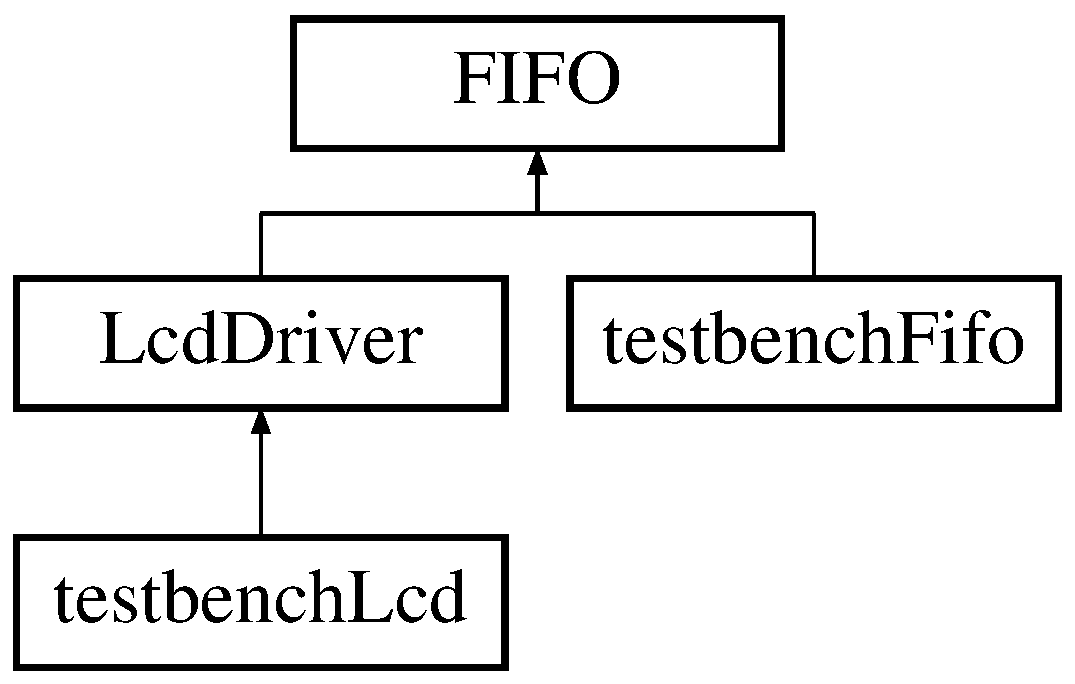
\includegraphics[height=3.000000cm]{classFIFO}
\end{center}
\end{figure}
\subsection*{Entities}
\begin{DoxyCompactItemize}
\item 
\hyperlink{classFIFO_1_1behavioural}{behavioural} architecture
\end{DoxyCompactItemize}
\subsection*{Libraries}
 \begin{DoxyCompactItemize}
\item 
\mbox{\Hypertarget{classFIFO_a0a6af6eef40212dbaf130d57ce711256}\label{classFIFO_a0a6af6eef40212dbaf130d57ce711256}} 
\hyperlink{classFIFO_a0a6af6eef40212dbaf130d57ce711256}{ieee} 
\end{DoxyCompactItemize}
\subsection*{Use Clauses}
 \begin{DoxyCompactItemize}
\item 
\mbox{\Hypertarget{classFIFO_acd03516902501cd1c7296a98e22c6fcb}\label{classFIFO_acd03516902501cd1c7296a98e22c6fcb}} 
\hyperlink{classFIFO_acd03516902501cd1c7296a98e22c6fcb}{std\+\_\+logic\+\_\+1164}   
\item 
\mbox{\Hypertarget{classFIFO_a2edc34402b573437d5f25fa90ba4013e}\label{classFIFO_a2edc34402b573437d5f25fa90ba4013e}} 
\hyperlink{classFIFO_a2edc34402b573437d5f25fa90ba4013e}{numeric\+\_\+std}   
\item 
\mbox{\Hypertarget{classFIFO_a598da929e807d58939b47499e8bc9fa8}\label{classFIFO_a598da929e807d58939b47499e8bc9fa8}} 
\hyperlink{classFIFO_a598da929e807d58939b47499e8bc9fa8}{std\+\_\+logic\+\_\+unsigned}   
\end{DoxyCompactItemize}
\subsection*{Generics}
 \begin{DoxyCompactItemize}
\item 
\mbox{\Hypertarget{classFIFO_ad061e94816abc61306c720c7ed29868b}\label{classFIFO_ad061e94816abc61306c720c7ed29868b}} 
\hyperlink{classFIFO_ad061e94816abc61306c720c7ed29868b}{S\+I\+ZE} {\bfseries {\bfseries \textcolor{vhdlchar}{natural}\textcolor{vhdlchar}{ }\textcolor{vhdlchar}{ }\textcolor{vhdlchar}{\+:}\textcolor{vhdlchar}{=}\textcolor{vhdlchar}{ }\textcolor{vhdlchar}{ } \textcolor{vhdldigit}{256} \textcolor{vhdlchar}{ }}}
\end{DoxyCompactItemize}
\subsection*{Ports}
 \begin{DoxyCompactItemize}
\item 
\mbox{\Hypertarget{classFIFO_a868bf8dd825e7fe9c3b5451faf25fcdf}\label{classFIFO_a868bf8dd825e7fe9c3b5451faf25fcdf}} 
\hyperlink{classFIFO_a868bf8dd825e7fe9c3b5451faf25fcdf}{Clk\+\_\+\+CI}  {\bfseries {\bfseries \textcolor{vhdlchar}{in}\textcolor{vhdlchar}{ }}} {\bfseries \textcolor{vhdlchar}{std\+\_\+logic}\textcolor{vhdlchar}{ }} 
\item 
\mbox{\Hypertarget{classFIFO_a9fcad7cb4e06dd5b58962adf49f7cbe5}\label{classFIFO_a9fcad7cb4e06dd5b58962adf49f7cbe5}} 
\hyperlink{classFIFO_a9fcad7cb4e06dd5b58962adf49f7cbe5}{Reset\+\_\+\+N\+RI}  {\bfseries {\bfseries \textcolor{vhdlchar}{in}\textcolor{vhdlchar}{ }}} {\bfseries \textcolor{vhdlchar}{std\+\_\+logic}\textcolor{vhdlchar}{ }} 
\item 
\mbox{\Hypertarget{classFIFO_a277e5650b931703d93c80248b7026b61}\label{classFIFO_a277e5650b931703d93c80248b7026b61}} 
\hyperlink{classFIFO_a277e5650b931703d93c80248b7026b61}{Push\+\_\+\+SI}  {\bfseries {\bfseries \textcolor{vhdlchar}{in}\textcolor{vhdlchar}{ }}} {\bfseries \textcolor{vhdlchar}{std\+\_\+logic}\textcolor{vhdlchar}{ }} 
\item 
\mbox{\Hypertarget{classFIFO_a1400289b3d87026371457d18f5a08585}\label{classFIFO_a1400289b3d87026371457d18f5a08585}} 
\hyperlink{classFIFO_a1400289b3d87026371457d18f5a08585}{Pop\+\_\+\+SI}  {\bfseries {\bfseries \textcolor{vhdlchar}{in}\textcolor{vhdlchar}{ }}} {\bfseries \textcolor{vhdlchar}{std\+\_\+logic}\textcolor{vhdlchar}{ }} 
\item 
\mbox{\Hypertarget{classFIFO_a7829d665526a19c3acd3771da7af2bee}\label{classFIFO_a7829d665526a19c3acd3771da7af2bee}} 
\hyperlink{classFIFO_a7829d665526a19c3acd3771da7af2bee}{Data\+\_\+\+DI}  {\bfseries {\bfseries \textcolor{vhdlchar}{in}\textcolor{vhdlchar}{ }}} {\bfseries \textcolor{vhdlchar}{std\+\_\+logic\+\_\+vector}\textcolor{vhdlchar}{ }\textcolor{vhdlchar}{(}\textcolor{vhdlchar}{ }\textcolor{vhdlchar}{ } \textcolor{vhdldigit}{15} \textcolor{vhdlchar}{ }\textcolor{vhdlchar}{downto}\textcolor{vhdlchar}{ }\textcolor{vhdlchar}{ } \textcolor{vhdldigit}{0} \textcolor{vhdlchar}{ }\textcolor{vhdlchar}{)}\textcolor{vhdlchar}{ }} 
\item 
\mbox{\Hypertarget{classFIFO_a7c4e766eeb918531625ac7d114bbc587}\label{classFIFO_a7c4e766eeb918531625ac7d114bbc587}} 
\hyperlink{classFIFO_a7c4e766eeb918531625ac7d114bbc587}{Data\+\_\+\+DO}  {\bfseries {\bfseries \textcolor{vhdlchar}{out}\textcolor{vhdlchar}{ }}} {\bfseries \textcolor{vhdlchar}{std\+\_\+logic\+\_\+vector}\textcolor{vhdlchar}{ }\textcolor{vhdlchar}{(}\textcolor{vhdlchar}{ }\textcolor{vhdlchar}{ } \textcolor{vhdldigit}{15} \textcolor{vhdlchar}{ }\textcolor{vhdlchar}{downto}\textcolor{vhdlchar}{ }\textcolor{vhdlchar}{ } \textcolor{vhdldigit}{0} \textcolor{vhdlchar}{ }\textcolor{vhdlchar}{)}\textcolor{vhdlchar}{ }} 
\item 
\mbox{\Hypertarget{classFIFO_a4532243c467861ba189f3da46dc354e9}\label{classFIFO_a4532243c467861ba189f3da46dc354e9}} 
\hyperlink{classFIFO_a4532243c467861ba189f3da46dc354e9}{Full\+\_\+\+SO}  {\bfseries {\bfseries \textcolor{vhdlchar}{out}\textcolor{vhdlchar}{ }}} {\bfseries \textcolor{vhdlchar}{std\+\_\+logic}\textcolor{vhdlchar}{ }} 
\item 
\mbox{\Hypertarget{classFIFO_afc033ac2b25da2bcb58a7d1a7fee0c9b}\label{classFIFO_afc033ac2b25da2bcb58a7d1a7fee0c9b}} 
\hyperlink{classFIFO_afc033ac2b25da2bcb58a7d1a7fee0c9b}{Empty\+\_\+\+SO}  {\bfseries {\bfseries \textcolor{vhdlchar}{out}\textcolor{vhdlchar}{ }}} {\bfseries \textcolor{vhdlchar}{std\+\_\+logic}\textcolor{vhdlchar}{ }} 
\end{DoxyCompactItemize}


The documentation for this class was generated from the following file\+:\begin{DoxyCompactItemize}
\item 
fifo.\+vhdl\end{DoxyCompactItemize}

\hypertarget{classLcdDriver_1_1LCD}{}\section{L\+CD Architecture Reference}
\label{classLcdDriver_1_1LCD}\index{L\+CD@{L\+CD}}
\subsection*{Processes}
 \begin{DoxyCompactItemize}
\item 
\mbox{\Hypertarget{classLcdDriver_1_1LCD_a8ddfdcf7d5753d2b8a763c46b1f66ede}\label{classLcdDriver_1_1LCD_a8ddfdcf7d5753d2b8a763c46b1f66ede}} 
\hyperlink{classLcdDriver_1_1LCD_a8ddfdcf7d5753d2b8a763c46b1f66ede}{edge\+Detect}{\bfseries  ( {\bfseries \textcolor{vhdlchar}{Reset\+\_\+\+N\+RI}\textcolor{vhdlchar}{ }} , {\bfseries \textcolor{vhdlchar}{Clk\+\_\+\+CI}\textcolor{vhdlchar}{ }} )}
\item 
\mbox{\Hypertarget{classLcdDriver_1_1LCD_a220a6885d47f04cad3e5b2a6f1528fd7}\label{classLcdDriver_1_1LCD_a220a6885d47f04cad3e5b2a6f1528fd7}} 
\hyperlink{classLcdDriver_1_1LCD_a220a6885d47f04cad3e5b2a6f1528fd7}{next\+State\+Rx}{\bfseries  ( {\bfseries \textcolor{vhdlchar}{Clk\+\_\+\+CI}\textcolor{vhdlchar}{ }} , {\bfseries \textcolor{vhdlchar}{Reset\+\_\+\+N\+RI}\textcolor{vhdlchar}{ }} )}
\item 
\mbox{\Hypertarget{classLcdDriver_1_1LCD_af3c0d0502a4e6217e00a6144a519144b}\label{classLcdDriver_1_1LCD_af3c0d0502a4e6217e00a6144a519144b}} 
\hyperlink{classLcdDriver_1_1LCD_af3c0d0502a4e6217e00a6144a519144b}{logic\+Rx}{\bfseries  ( {\bfseries \textcolor{vhdlchar}{Clk\+\_\+\+CI}\textcolor{vhdlchar}{ }} , {\bfseries \textcolor{vhdlchar}{Rx\+State\+Pres\+\_\+D}\textcolor{vhdlchar}{ }} , {\bfseries \textcolor{vhdlchar}{Fifo\+Full\+\_\+D}\textcolor{vhdlchar}{ }} , {\bfseries \textcolor{vhdlchar}{Write\+\_\+\+Edge\+\_\+D}\textcolor{vhdlchar}{ }} , {\bfseries \textcolor{vhdlchar}{Rx\+Data\+\_\+D}\textcolor{vhdlchar}{ }} )}
\item 
\mbox{\Hypertarget{classLcdDriver_1_1LCD_a53afafce4de3dcf2709153c18013d0c6}\label{classLcdDriver_1_1LCD_a53afafce4de3dcf2709153c18013d0c6}} 
\hyperlink{classLcdDriver_1_1LCD_a53afafce4de3dcf2709153c18013d0c6}{next\+State\+Tx}{\bfseries  ( {\bfseries \textcolor{vhdlchar}{Clk\+\_\+\+CI}\textcolor{vhdlchar}{ }} , {\bfseries \textcolor{vhdlchar}{Reset\+\_\+\+N\+RI}\textcolor{vhdlchar}{ }} )}
\item 
\mbox{\Hypertarget{classLcdDriver_1_1LCD_acd55b2e2a62219eec4bba8d508e1ffe3}\label{classLcdDriver_1_1LCD_acd55b2e2a62219eec4bba8d508e1ffe3}} 
\hyperlink{classLcdDriver_1_1LCD_acd55b2e2a62219eec4bba8d508e1ffe3}{logic\+Tx}{\bfseries  ( {\bfseries \textcolor{vhdlchar}{Clk\+\_\+\+CI}\textcolor{vhdlchar}{ }} , {\bfseries \textcolor{vhdlchar}{Tx\+State\+Pres\+\_\+D}\textcolor{vhdlchar}{ }} , {\bfseries \textcolor{vhdlchar}{Fifo\+Empty\+\_\+D}\textcolor{vhdlchar}{ }} )}
\end{DoxyCompactItemize}
\subsection*{Components}
 \begin{DoxyCompactItemize}
\item 
\mbox{\Hypertarget{classLcdDriver_1_1LCD_a2055ffc86a781cfd9d1470f72494f04a}\label{classLcdDriver_1_1LCD_a2055ffc86a781cfd9d1470f72494f04a}} 
\hyperlink{classLcdDriver_1_1LCD_a2055ffc86a781cfd9d1470f72494f04a}{F\+I\+FO}  {\bfseries }  
\end{DoxyCompactItemize}
\subsection*{Types}
 \begin{DoxyCompactItemize}
\item 
\mbox{\Hypertarget{classLcdDriver_1_1LCD_a36ab1b4afe84944ea4c18e7a0e0b4cea}\label{classLcdDriver_1_1LCD_a36ab1b4afe84944ea4c18e7a0e0b4cea}} 
{\bfseries \hyperlink{classLcdDriver_1_1LCD_a36ab1b4afe84944ea4c18e7a0e0b4cea}{Rx\+State\+\_\+T}{\bfseries \textcolor{vhdlchar}{(}\textcolor{vhdlchar}{ }\textcolor{vhdlchar}{Rx\+State\+Reset}\textcolor{vhdlchar}{ }\textcolor{vhdlchar}{,}\textcolor{vhdlchar}{ }\textcolor{vhdlchar}{Rx\+State\+Idle}\textcolor{vhdlchar}{ }\textcolor{vhdlchar}{,}\textcolor{vhdlchar}{ }\textcolor{vhdlchar}{Rx\+State\+Rx\+Pre\+Push\+Cmd}\textcolor{vhdlchar}{ }\textcolor{vhdlchar}{,}\textcolor{vhdlchar}{ }\textcolor{vhdlchar}{Rx\+State\+Rx\+Pre\+Push\+Data\+Identifier}\textcolor{vhdlchar}{ }\textcolor{vhdlchar}{,}\textcolor{vhdlchar}{ }\textcolor{vhdlchar}{Rx\+State\+Rx\+Pre\+Push\+Data}\textcolor{vhdlchar}{ }\textcolor{vhdlchar}{,}\textcolor{vhdlchar}{ }\textcolor{vhdlchar}{Rx\+State\+Rx\+Post\+Push\+Data\+Identifier}\textcolor{vhdlchar}{ }\textcolor{vhdlchar}{,}\textcolor{vhdlchar}{ }\textcolor{vhdlchar}{Rx\+State\+Rx\+Post\+Push}\textcolor{vhdlchar}{ }\textcolor{vhdlchar}{)}\textcolor{vhdlchar}{ }}} 
\item 
\mbox{\Hypertarget{classLcdDriver_1_1LCD_a72cbc922b8204936ec69fa7acbbf5140}\label{classLcdDriver_1_1LCD_a72cbc922b8204936ec69fa7acbbf5140}} 
{\bfseries \hyperlink{classLcdDriver_1_1LCD_a72cbc922b8204936ec69fa7acbbf5140}{Tx\+State\+\_\+T}{\bfseries \textcolor{vhdlchar}{(}\textcolor{vhdlchar}{ }\textcolor{vhdlchar}{Tx\+State\+Reset}\textcolor{vhdlchar}{ }\textcolor{vhdlchar}{,}\textcolor{vhdlchar}{ }\textcolor{vhdlchar}{Tx\+State\+Disp\+Reset}\textcolor{vhdlchar}{ }\textcolor{vhdlchar}{,}\textcolor{vhdlchar}{ }\textcolor{vhdlchar}{Tx\+State\+Idle}\textcolor{vhdlchar}{ }\textcolor{vhdlchar}{,}\textcolor{vhdlchar}{ }\textcolor{vhdlchar}{Tx\+State\+Pre\+Tx}\textcolor{vhdlchar}{ }\textcolor{vhdlchar}{,}\textcolor{vhdlchar}{ }\textcolor{vhdlchar}{Tx\+State\+Tx}\textcolor{vhdlchar}{ }\textcolor{vhdlchar}{,}\textcolor{vhdlchar}{ }\textcolor{vhdlchar}{Tx\+State\+Post\+Tx}\textcolor{vhdlchar}{ }\textcolor{vhdlchar}{)}\textcolor{vhdlchar}{ }}} 
\end{DoxyCompactItemize}
\subsection*{Signals}
 \begin{DoxyCompactItemize}
\item 
\mbox{\Hypertarget{classLcdDriver_1_1LCD_ad7a80173a124881de64345b464848cec}\label{classLcdDriver_1_1LCD_ad7a80173a124881de64345b464848cec}} 
\hyperlink{classLcdDriver_1_1LCD_ad7a80173a124881de64345b464848cec}{Rx\+State\+Next\+\_\+D} {\bfseries \textcolor{vhdlchar}{Rx\+State\+\_\+T}\textcolor{vhdlchar}{ }\textcolor{vhdlchar}{ }\textcolor{vhdlchar}{\+:}\textcolor{vhdlchar}{=}\textcolor{vhdlchar}{ }\textcolor{vhdlchar}{ }\textcolor{vhdlchar}{ }\textcolor{vhdlchar}{ }\textcolor{vhdlchar}{Rx\+State\+Reset}\textcolor{vhdlchar}{ }} 
\item 
\mbox{\Hypertarget{classLcdDriver_1_1LCD_a4f383b2ed07478e8160c0d3c6ef246df}\label{classLcdDriver_1_1LCD_a4f383b2ed07478e8160c0d3c6ef246df}} 
\hyperlink{classLcdDriver_1_1LCD_a4f383b2ed07478e8160c0d3c6ef246df}{Tx\+State\+Next\+\_\+D} {\bfseries \textcolor{vhdlchar}{Tx\+State\+\_\+T}\textcolor{vhdlchar}{ }\textcolor{vhdlchar}{ }\textcolor{vhdlchar}{\+:}\textcolor{vhdlchar}{=}\textcolor{vhdlchar}{ }\textcolor{vhdlchar}{ }\textcolor{vhdlchar}{ }\textcolor{vhdlchar}{ }\textcolor{vhdlchar}{Tx\+S\+Tate\+Reset}\textcolor{vhdlchar}{ }} 
\item 
\mbox{\Hypertarget{classLcdDriver_1_1LCD_a3829b589f0b8cf0c0a8705c0a4d2ec4d}\label{classLcdDriver_1_1LCD_a3829b589f0b8cf0c0a8705c0a4d2ec4d}} 
\hyperlink{classLcdDriver_1_1LCD_a3829b589f0b8cf0c0a8705c0a4d2ec4d}{Rx\+State\+Pres\+\_\+D} {\bfseries \textcolor{vhdlchar}{Rx\+State\+\_\+T}\textcolor{vhdlchar}{ }\textcolor{vhdlchar}{ }\textcolor{vhdlchar}{\+:}\textcolor{vhdlchar}{=}\textcolor{vhdlchar}{ }\textcolor{vhdlchar}{ }\textcolor{vhdlchar}{ }\textcolor{vhdlchar}{ }\textcolor{vhdlchar}{Rx\+State\+Reset}\textcolor{vhdlchar}{ }} 
\item 
\mbox{\Hypertarget{classLcdDriver_1_1LCD_a2fb0f12e314d4b763327137313083d6a}\label{classLcdDriver_1_1LCD_a2fb0f12e314d4b763327137313083d6a}} 
\hyperlink{classLcdDriver_1_1LCD_a2fb0f12e314d4b763327137313083d6a}{Tx\+State\+Pres\+\_\+D} {\bfseries \textcolor{vhdlchar}{Tx\+State\+\_\+T}\textcolor{vhdlchar}{ }\textcolor{vhdlchar}{ }\textcolor{vhdlchar}{\+:}\textcolor{vhdlchar}{=}\textcolor{vhdlchar}{ }\textcolor{vhdlchar}{ }\textcolor{vhdlchar}{ }\textcolor{vhdlchar}{ }\textcolor{vhdlchar}{Tx\+S\+Tate\+Reset}\textcolor{vhdlchar}{ }} 
\item 
\mbox{\Hypertarget{classLcdDriver_1_1LCD_a20c382c54ed3a8ea50dd2533a5379bf1}\label{classLcdDriver_1_1LCD_a20c382c54ed3a8ea50dd2533a5379bf1}} 
\hyperlink{classLcdDriver_1_1LCD_a20c382c54ed3a8ea50dd2533a5379bf1}{Pop\+\_\+S} {\bfseries \textcolor{vhdlchar}{std\+\_\+logic}\textcolor{vhdlchar}{ }} 
\item 
\mbox{\Hypertarget{classLcdDriver_1_1LCD_a0ee8a6f0f033cba23759470b8791e722}\label{classLcdDriver_1_1LCD_a0ee8a6f0f033cba23759470b8791e722}} 
\hyperlink{classLcdDriver_1_1LCD_a0ee8a6f0f033cba23759470b8791e722}{Push\+\_\+S} {\bfseries \textcolor{vhdlchar}{std\+\_\+logic}\textcolor{vhdlchar}{ }} 
\item 
\mbox{\Hypertarget{classLcdDriver_1_1LCD_ac21e8b1a5fe90e1579752fd40e6ca14a}\label{classLcdDriver_1_1LCD_ac21e8b1a5fe90e1579752fd40e6ca14a}} 
\hyperlink{classLcdDriver_1_1LCD_ac21e8b1a5fe90e1579752fd40e6ca14a}{Rx\+Data\+\_\+D} {\bfseries \textcolor{vhdlchar}{std\+\_\+logic\+\_\+vector}\textcolor{vhdlchar}{ }\textcolor{vhdlchar}{(}\textcolor{vhdlchar}{ }\textcolor{vhdlchar}{ } \textcolor{vhdldigit}{15} \textcolor{vhdlchar}{ }\textcolor{vhdlchar}{downto}\textcolor{vhdlchar}{ }\textcolor{vhdlchar}{ } \textcolor{vhdldigit}{0} \textcolor{vhdlchar}{ }\textcolor{vhdlchar}{)}\textcolor{vhdlchar}{ }} 
\item 
\mbox{\Hypertarget{classLcdDriver_1_1LCD_a8719487972d6ccf8abe0e450b65427ee}\label{classLcdDriver_1_1LCD_a8719487972d6ccf8abe0e450b65427ee}} 
\hyperlink{classLcdDriver_1_1LCD_a8719487972d6ccf8abe0e450b65427ee}{Tx\+Data\+\_\+D} {\bfseries \textcolor{vhdlchar}{std\+\_\+logic\+\_\+vector}\textcolor{vhdlchar}{ }\textcolor{vhdlchar}{(}\textcolor{vhdlchar}{ }\textcolor{vhdlchar}{ } \textcolor{vhdldigit}{15} \textcolor{vhdlchar}{ }\textcolor{vhdlchar}{downto}\textcolor{vhdlchar}{ }\textcolor{vhdlchar}{ } \textcolor{vhdldigit}{0} \textcolor{vhdlchar}{ }\textcolor{vhdlchar}{)}\textcolor{vhdlchar}{ }} 
\item 
\mbox{\Hypertarget{classLcdDriver_1_1LCD_aad1f8bd3de5c8d177201363617714542}\label{classLcdDriver_1_1LCD_aad1f8bd3de5c8d177201363617714542}} 
\hyperlink{classLcdDriver_1_1LCD_aad1f8bd3de5c8d177201363617714542}{Fifo\+Full\+\_\+D} {\bfseries \textcolor{vhdlchar}{std\+\_\+logic}\textcolor{vhdlchar}{ }} 
\item 
\mbox{\Hypertarget{classLcdDriver_1_1LCD_a8bc39f88133f2d60b389e86590df812f}\label{classLcdDriver_1_1LCD_a8bc39f88133f2d60b389e86590df812f}} 
\hyperlink{classLcdDriver_1_1LCD_a8bc39f88133f2d60b389e86590df812f}{Fifo\+Empty\+\_\+D} {\bfseries \textcolor{vhdlchar}{std\+\_\+logic}\textcolor{vhdlchar}{ }} 
\item 
\mbox{\Hypertarget{classLcdDriver_1_1LCD_a520390c4bac9e8d56530e87a3757221d}\label{classLcdDriver_1_1LCD_a520390c4bac9e8d56530e87a3757221d}} 
\hyperlink{classLcdDriver_1_1LCD_a520390c4bac9e8d56530e87a3757221d}{Is\+Data\+\_\+D} {\bfseries \textcolor{vhdlchar}{std\+\_\+logic}\textcolor{vhdlchar}{ }} 
\item 
\mbox{\Hypertarget{classLcdDriver_1_1LCD_a1fdded4d7a1bd30bf7bb065751b5d3bd}\label{classLcdDriver_1_1LCD_a1fdded4d7a1bd30bf7bb065751b5d3bd}} 
\hyperlink{classLcdDriver_1_1LCD_a1fdded4d7a1bd30bf7bb065751b5d3bd}{Bit\+Enable\+\_\+D} {\bfseries \textcolor{vhdlchar}{std\+\_\+logic\+\_\+vector}\textcolor{vhdlchar}{ }\textcolor{vhdlchar}{(}\textcolor{vhdlchar}{ }\textcolor{vhdlchar}{ } \textcolor{vhdldigit}{15} \textcolor{vhdlchar}{ }\textcolor{vhdlchar}{downto}\textcolor{vhdlchar}{ }\textcolor{vhdlchar}{ } \textcolor{vhdldigit}{0} \textcolor{vhdlchar}{ }\textcolor{vhdlchar}{)}\textcolor{vhdlchar}{ }} 
\item 
\mbox{\Hypertarget{classLcdDriver_1_1LCD_a13084956378e5d1870a120551cdcc15e}\label{classLcdDriver_1_1LCD_a13084956378e5d1870a120551cdcc15e}} 
\hyperlink{classLcdDriver_1_1LCD_a13084956378e5d1870a120551cdcc15e}{Write\+\_\+\+Edge\+\_\+D} {\bfseries \textcolor{vhdlchar}{std\+\_\+logic}\textcolor{vhdlchar}{ }} 
\item 
\mbox{\Hypertarget{classLcdDriver_1_1LCD_aa636d0a07fe3d651bc4ff7bfd3cbcd1b}\label{classLcdDriver_1_1LCD_aa636d0a07fe3d651bc4ff7bfd3cbcd1b}} 
\hyperlink{classLcdDriver_1_1LCD_aa636d0a07fe3d651bc4ff7bfd3cbcd1b}{Write\+\_\+\+Last\+\_\+D} {\bfseries \textcolor{vhdlchar}{std\+\_\+logic}\textcolor{vhdlchar}{ }} 
\item 
\mbox{\Hypertarget{classLcdDriver_1_1LCD_a5f2bd27dbd5322df7874cc38de794d6e}\label{classLcdDriver_1_1LCD_a5f2bd27dbd5322df7874cc38de794d6e}} 
\hyperlink{classLcdDriver_1_1LCD_a5f2bd27dbd5322df7874cc38de794d6e}{Read\+\_\+\+Edge\+\_\+D} {\bfseries \textcolor{vhdlchar}{std\+\_\+logic}\textcolor{vhdlchar}{ }} 
\item 
\mbox{\Hypertarget{classLcdDriver_1_1LCD_a3c0fa31aacd37b70ca2fd7b289cecbb9}\label{classLcdDriver_1_1LCD_a3c0fa31aacd37b70ca2fd7b289cecbb9}} 
\hyperlink{classLcdDriver_1_1LCD_a3c0fa31aacd37b70ca2fd7b289cecbb9}{Read\+\_\+\+Last\+\_\+D} {\bfseries \textcolor{vhdlchar}{std\+\_\+logic}\textcolor{vhdlchar}{ }} 
\end{DoxyCompactItemize}
\subsection*{Instantiations}
 \begin{DoxyCompactItemize}
\item 
\mbox{\Hypertarget{classLcdDriver_1_1LCD_a29d3add4a26a57750813a567c58e23b1}\label{classLcdDriver_1_1LCD_a29d3add4a26a57750813a567c58e23b1}} 
\hyperlink{classLcdDriver_1_1LCD_a29d3add4a26a57750813a567c58e23b1}{databuffer}  {\bfseries F\+I\+FO}   
\end{DoxyCompactItemize}


The documentation for this class was generated from the following file\+:\begin{DoxyCompactItemize}
\item 
\hyperlink{lcdDriver_8vhdl}{lcd\+Driver.\+vhdl}\end{DoxyCompactItemize}

\hypertarget{classLcdDriver}{}\section{Lcd\+Driver Entity Reference}
\label{classLcdDriver}\index{Lcd\+Driver@{Lcd\+Driver}}
Inheritance diagram for Lcd\+Driver\+:\begin{figure}[H]
\begin{center}
\leavevmode
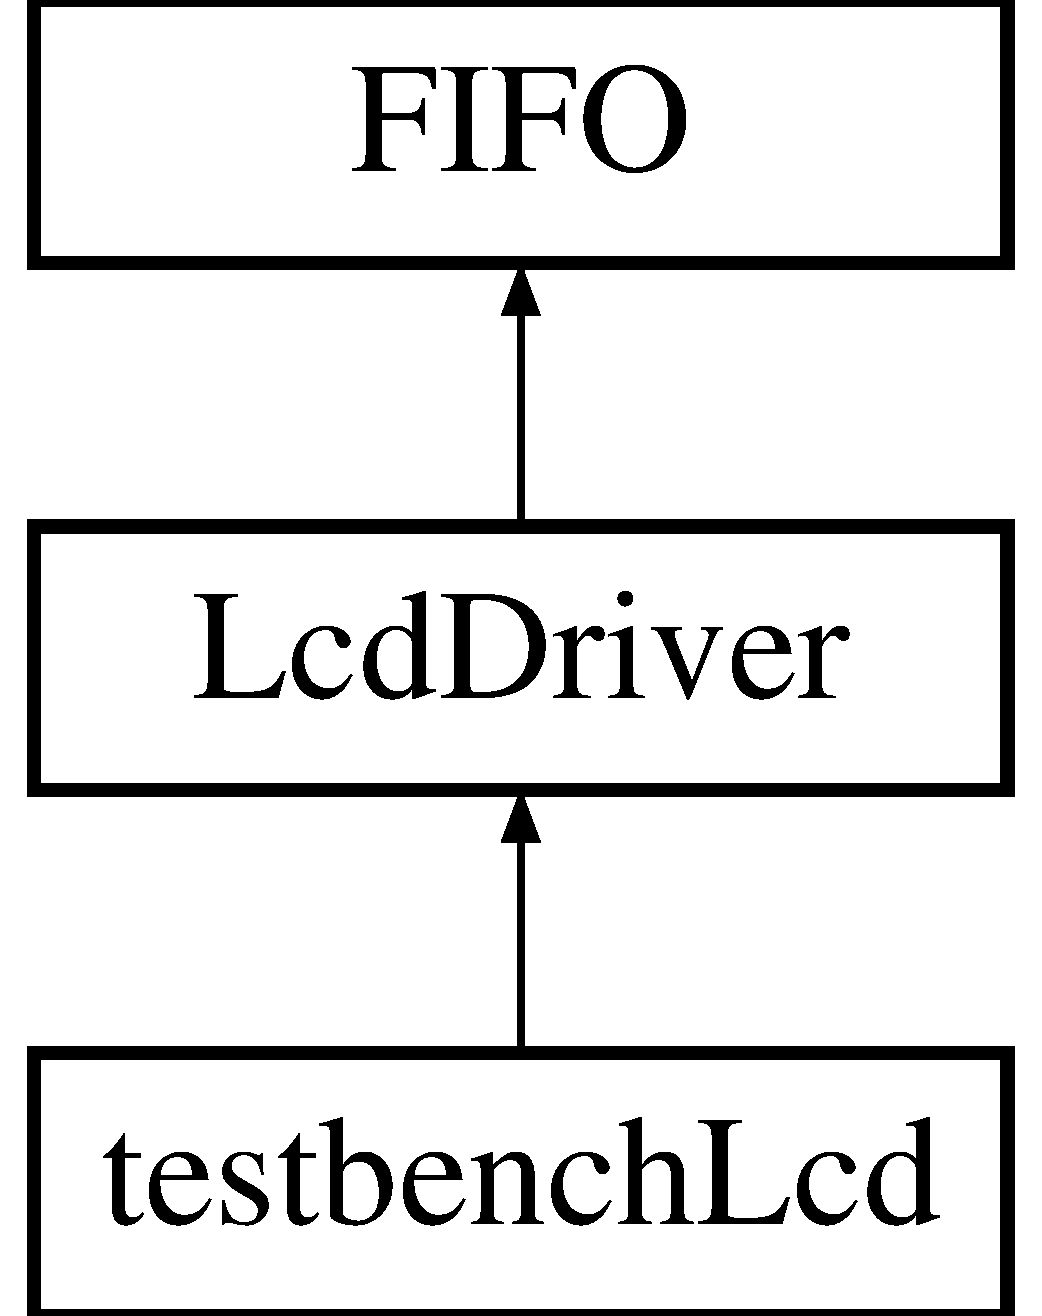
\includegraphics[height=3.000000cm]{classLcdDriver}
\end{center}
\end{figure}
\subsection*{Entities}
\begin{DoxyCompactItemize}
\item 
\hyperlink{classLcdDriver_1_1LCD}{L\+CD} architecture
\end{DoxyCompactItemize}
\subsection*{Libraries}
 \begin{DoxyCompactItemize}
\item 
\mbox{\Hypertarget{classLcdDriver_a0a6af6eef40212dbaf130d57ce711256}\label{classLcdDriver_a0a6af6eef40212dbaf130d57ce711256}} 
\hyperlink{classLcdDriver_a0a6af6eef40212dbaf130d57ce711256}{ieee} 
\end{DoxyCompactItemize}
\subsection*{Use Clauses}
 \begin{DoxyCompactItemize}
\item 
\mbox{\Hypertarget{classLcdDriver_acd03516902501cd1c7296a98e22c6fcb}\label{classLcdDriver_acd03516902501cd1c7296a98e22c6fcb}} 
\hyperlink{classLcdDriver_acd03516902501cd1c7296a98e22c6fcb}{std\+\_\+logic\+\_\+1164}   
\item 
\mbox{\Hypertarget{classLcdDriver_a2edc34402b573437d5f25fa90ba4013e}\label{classLcdDriver_a2edc34402b573437d5f25fa90ba4013e}} 
\hyperlink{classLcdDriver_a2edc34402b573437d5f25fa90ba4013e}{numeric\+\_\+std}   
\end{DoxyCompactItemize}
\subsection*{Ports}
 \begin{DoxyCompactItemize}
\item 
\mbox{\Hypertarget{classLcdDriver_a868bf8dd825e7fe9c3b5451faf25fcdf}\label{classLcdDriver_a868bf8dd825e7fe9c3b5451faf25fcdf}} 
\hyperlink{classLcdDriver_a868bf8dd825e7fe9c3b5451faf25fcdf}{Clk\+\_\+\+CI}  {\bfseries {\bfseries \textcolor{vhdlchar}{in}\textcolor{vhdlchar}{ }}} {\bfseries \textcolor{vhdlchar}{std\+\_\+logic}\textcolor{vhdlchar}{ }} 
\item 
\mbox{\Hypertarget{classLcdDriver_a9fcad7cb4e06dd5b58962adf49f7cbe5}\label{classLcdDriver_a9fcad7cb4e06dd5b58962adf49f7cbe5}} 
\hyperlink{classLcdDriver_a9fcad7cb4e06dd5b58962adf49f7cbe5}{Reset\+\_\+\+N\+RI}  {\bfseries {\bfseries \textcolor{vhdlchar}{in}\textcolor{vhdlchar}{ }}} {\bfseries \textcolor{vhdlchar}{std\+\_\+logic}\textcolor{vhdlchar}{ }} 
\item 
\mbox{\Hypertarget{classLcdDriver_addb9eba0cb0fed127cba182475244260}\label{classLcdDriver_addb9eba0cb0fed127cba182475244260}} 
\hyperlink{classLcdDriver_addb9eba0cb0fed127cba182475244260}{Address\+\_\+\+DI}  {\bfseries {\bfseries \textcolor{vhdlchar}{in}\textcolor{vhdlchar}{ }}} {\bfseries \textcolor{vhdlchar}{std\+\_\+logic\+\_\+vector}\textcolor{vhdlchar}{ }\textcolor{vhdlchar}{(}\textcolor{vhdlchar}{ }\textcolor{vhdlchar}{ } \textcolor{vhdldigit}{1} \textcolor{vhdlchar}{ }\textcolor{vhdlchar}{downto}\textcolor{vhdlchar}{ }\textcolor{vhdlchar}{ } \textcolor{vhdldigit}{0} \textcolor{vhdlchar}{ }\textcolor{vhdlchar}{)}\textcolor{vhdlchar}{ }} 
\item 
\mbox{\Hypertarget{classLcdDriver_a159dd0ab062d7714a5e7e4478bcb201e}\label{classLcdDriver_a159dd0ab062d7714a5e7e4478bcb201e}} 
\hyperlink{classLcdDriver_a159dd0ab062d7714a5e7e4478bcb201e}{Write\+\_\+\+SI}  {\bfseries {\bfseries \textcolor{vhdlchar}{in}\textcolor{vhdlchar}{ }}} {\bfseries \textcolor{vhdlchar}{std\+\_\+logic}\textcolor{vhdlchar}{ }} 
\item 
\mbox{\Hypertarget{classLcdDriver_a9fa1024d06a6ae0556c7f71e0900f3a9}\label{classLcdDriver_a9fa1024d06a6ae0556c7f71e0900f3a9}} 
\hyperlink{classLcdDriver_a9fa1024d06a6ae0556c7f71e0900f3a9}{Write\+Data\+\_\+\+DI}  {\bfseries {\bfseries \textcolor{vhdlchar}{in}\textcolor{vhdlchar}{ }}} {\bfseries \textcolor{vhdlchar}{std\+\_\+logic\+\_\+vector}\textcolor{vhdlchar}{ }\textcolor{vhdlchar}{(}\textcolor{vhdlchar}{ }\textcolor{vhdlchar}{ } \textcolor{vhdldigit}{15} \textcolor{vhdlchar}{ }\textcolor{vhdlchar}{downto}\textcolor{vhdlchar}{ }\textcolor{vhdlchar}{ } \textcolor{vhdldigit}{0} \textcolor{vhdlchar}{ }\textcolor{vhdlchar}{)}\textcolor{vhdlchar}{ }} 
\item 
\mbox{\Hypertarget{classLcdDriver_a43f227fe462eb1ae9a41cd6f60ba3afb}\label{classLcdDriver_a43f227fe462eb1ae9a41cd6f60ba3afb}} 
\hyperlink{classLcdDriver_a43f227fe462eb1ae9a41cd6f60ba3afb}{Read\+\_\+\+SI}  {\bfseries {\bfseries \textcolor{vhdlchar}{in}\textcolor{vhdlchar}{ }}} {\bfseries \textcolor{vhdlchar}{std\+\_\+logic}\textcolor{vhdlchar}{ }} 
\item 
\mbox{\Hypertarget{classLcdDriver_ab72d07bf4471b0ac7d031956dd62e5db}\label{classLcdDriver_ab72d07bf4471b0ac7d031956dd62e5db}} 
\hyperlink{classLcdDriver_ab72d07bf4471b0ac7d031956dd62e5db}{Byte\+Enable\+\_\+\+DI}  {\bfseries {\bfseries \textcolor{vhdlchar}{in}\textcolor{vhdlchar}{ }}} {\bfseries \textcolor{vhdlchar}{std\+\_\+logic\+\_\+vector}\textcolor{vhdlchar}{ }\textcolor{vhdlchar}{(}\textcolor{vhdlchar}{ }\textcolor{vhdlchar}{ } \textcolor{vhdldigit}{1} \textcolor{vhdlchar}{ }\textcolor{vhdlchar}{downto}\textcolor{vhdlchar}{ }\textcolor{vhdlchar}{ } \textcolor{vhdldigit}{0} \textcolor{vhdlchar}{ }\textcolor{vhdlchar}{)}\textcolor{vhdlchar}{ }} 
\item 
\mbox{\Hypertarget{classLcdDriver_a091b01b8dedaf16f042d963740971d6a}\label{classLcdDriver_a091b01b8dedaf16f042d963740971d6a}} 
\hyperlink{classLcdDriver_a091b01b8dedaf16f042d963740971d6a}{Begin\+Burst\+Transfer\+\_\+\+DI}  {\bfseries {\bfseries \textcolor{vhdlchar}{in}\textcolor{vhdlchar}{ }}} {\bfseries \textcolor{vhdlchar}{std\+\_\+logic}\textcolor{vhdlchar}{ }} 
\item 
\mbox{\Hypertarget{classLcdDriver_adb5e34d589abfe19a4195988abd4f80f}\label{classLcdDriver_adb5e34d589abfe19a4195988abd4f80f}} 
\hyperlink{classLcdDriver_adb5e34d589abfe19a4195988abd4f80f}{Burst\+Count\+\_\+\+DI}  {\bfseries {\bfseries \textcolor{vhdlchar}{in}\textcolor{vhdlchar}{ }}} {\bfseries \textcolor{vhdlchar}{std\+\_\+logic\+\_\+vector}\textcolor{vhdlchar}{ }\textcolor{vhdlchar}{(}\textcolor{vhdlchar}{ }\textcolor{vhdlchar}{ } \textcolor{vhdldigit}{7} \textcolor{vhdlchar}{ }\textcolor{vhdlchar}{downto}\textcolor{vhdlchar}{ }\textcolor{vhdlchar}{ } \textcolor{vhdldigit}{0} \textcolor{vhdlchar}{ }\textcolor{vhdlchar}{)}\textcolor{vhdlchar}{ }} 
\item 
\mbox{\Hypertarget{classLcdDriver_a51e4b3eade0ceb0693d92043e9158ce0}\label{classLcdDriver_a51e4b3eade0ceb0693d92043e9158ce0}} 
\hyperlink{classLcdDriver_a51e4b3eade0ceb0693d92043e9158ce0}{Wait\+Req\+\_\+\+SO}  {\bfseries {\bfseries \textcolor{vhdlchar}{out}\textcolor{vhdlchar}{ }}} {\bfseries \textcolor{vhdlchar}{std\+\_\+logic}\textcolor{vhdlchar}{ }} 
\item 
\mbox{\Hypertarget{classLcdDriver_a866d91159c011d50505afa464f7dc531}\label{classLcdDriver_a866d91159c011d50505afa464f7dc531}} 
\hyperlink{classLcdDriver_a866d91159c011d50505afa464f7dc531}{Read\+Data\+\_\+\+DO}  {\bfseries {\bfseries \textcolor{vhdlchar}{out}\textcolor{vhdlchar}{ }}} {\bfseries \textcolor{vhdlchar}{std\+\_\+logic\+\_\+vector}\textcolor{vhdlchar}{ }\textcolor{vhdlchar}{(}\textcolor{vhdlchar}{ }\textcolor{vhdlchar}{ } \textcolor{vhdldigit}{15} \textcolor{vhdlchar}{ }\textcolor{vhdlchar}{downto}\textcolor{vhdlchar}{ }\textcolor{vhdlchar}{ } \textcolor{vhdldigit}{0} \textcolor{vhdlchar}{ }\textcolor{vhdlchar}{)}\textcolor{vhdlchar}{ }} 
\item 
\mbox{\Hypertarget{classLcdDriver_a336812155e41c9fbb2236431cfe4ec81}\label{classLcdDriver_a336812155e41c9fbb2236431cfe4ec81}} 
\hyperlink{classLcdDriver_a336812155e41c9fbb2236431cfe4ec81}{Read\+Data\+Valid\+\_\+\+SO}  {\bfseries {\bfseries \textcolor{vhdlchar}{out}\textcolor{vhdlchar}{ }}} {\bfseries \textcolor{vhdlchar}{std\+\_\+logic}\textcolor{vhdlchar}{ }} 
\item 
\mbox{\Hypertarget{classLcdDriver_aac95abbeb21e199184b2b994cc6e6641}\label{classLcdDriver_aac95abbeb21e199184b2b994cc6e6641}} 
\hyperlink{classLcdDriver_aac95abbeb21e199184b2b994cc6e6641}{D\+B\+\_\+\+D\+IO}  {\bfseries {\bfseries \textcolor{vhdlchar}{inout}\textcolor{vhdlchar}{ }}} {\bfseries \textcolor{vhdlchar}{std\+\_\+logic\+\_\+vector}\textcolor{vhdlchar}{ }\textcolor{vhdlchar}{(}\textcolor{vhdlchar}{ }\textcolor{vhdlchar}{ } \textcolor{vhdldigit}{15} \textcolor{vhdlchar}{ }\textcolor{vhdlchar}{downto}\textcolor{vhdlchar}{ }\textcolor{vhdlchar}{ } \textcolor{vhdldigit}{0} \textcolor{vhdlchar}{ }\textcolor{vhdlchar}{)}\textcolor{vhdlchar}{ }} 
\item 
\mbox{\Hypertarget{classLcdDriver_aac54d5bf05c3b78fe1551e006fd84cc8}\label{classLcdDriver_aac54d5bf05c3b78fe1551e006fd84cc8}} 
\hyperlink{classLcdDriver_aac54d5bf05c3b78fe1551e006fd84cc8}{Rd\+\_\+\+N\+SO}  {\bfseries {\bfseries \textcolor{vhdlchar}{out}\textcolor{vhdlchar}{ }}} {\bfseries \textcolor{vhdlchar}{std\+\_\+logic}\textcolor{vhdlchar}{ }} 
\item 
\mbox{\Hypertarget{classLcdDriver_a5de18cf676b22307e183dd8451913f76}\label{classLcdDriver_a5de18cf676b22307e183dd8451913f76}} 
\hyperlink{classLcdDriver_a5de18cf676b22307e183dd8451913f76}{Wr\+\_\+\+N\+SO}  {\bfseries {\bfseries \textcolor{vhdlchar}{out}\textcolor{vhdlchar}{ }}} {\bfseries \textcolor{vhdlchar}{std\+\_\+logic}\textcolor{vhdlchar}{ }} 
\item 
\mbox{\Hypertarget{classLcdDriver_ad7d8ed8b658f475fe5794db14cbf4756}\label{classLcdDriver_ad7d8ed8b658f475fe5794db14cbf4756}} 
\hyperlink{classLcdDriver_ad7d8ed8b658f475fe5794db14cbf4756}{Cs\+\_\+\+N\+SO}  {\bfseries {\bfseries \textcolor{vhdlchar}{out}\textcolor{vhdlchar}{ }}} {\bfseries \textcolor{vhdlchar}{std\+\_\+logic}\textcolor{vhdlchar}{ }} 
\item 
\mbox{\Hypertarget{classLcdDriver_a03ca52f19c4fbcc08c96833ffbbb8446}\label{classLcdDriver_a03ca52f19c4fbcc08c96833ffbbb8446}} 
\hyperlink{classLcdDriver_a03ca52f19c4fbcc08c96833ffbbb8446}{D\+C\+\_\+\+N\+SO}  {\bfseries {\bfseries \textcolor{vhdlchar}{out}\textcolor{vhdlchar}{ }}} {\bfseries \textcolor{vhdlchar}{std\+\_\+logic}\textcolor{vhdlchar}{ }} 
\item 
\mbox{\Hypertarget{classLcdDriver_a6e8b56885d3957111538a162097f51c1}\label{classLcdDriver_a6e8b56885d3957111538a162097f51c1}} 
\hyperlink{classLcdDriver_a6e8b56885d3957111538a162097f51c1}{Lcd\+Reset\+\_\+\+N\+RO}  {\bfseries {\bfseries \textcolor{vhdlchar}{out}\textcolor{vhdlchar}{ }}} {\bfseries \textcolor{vhdlchar}{std\+\_\+logic}\textcolor{vhdlchar}{ }} 
\item 
\mbox{\Hypertarget{classLcdDriver_a80c9d9678961bd65ade48155e55345b8}\label{classLcdDriver_a80c9d9678961bd65ade48155e55345b8}} 
\hyperlink{classLcdDriver_a80c9d9678961bd65ade48155e55345b8}{I\+M0\+\_\+\+SO}  {\bfseries {\bfseries \textcolor{vhdlchar}{out}\textcolor{vhdlchar}{ }}} {\bfseries \textcolor{vhdlchar}{std\+\_\+logic}\textcolor{vhdlchar}{ }} 
\end{DoxyCompactItemize}


The documentation for this class was generated from the following file\+:\begin{DoxyCompactItemize}
\item 
\hyperlink{lcdDriver_8vhdl}{lcd\+Driver.\+vhdl}\end{DoxyCompactItemize}

\hypertarget{classreader}{}\section{reader Entity Reference}
\label{classreader}\index{reader@{reader}}
\subsection*{Entities}
\begin{DoxyCompactItemize}
\item 
\hyperlink{classreader_1_1behavioural}{behavioural} architecture
\end{DoxyCompactItemize}
\subsection*{Libraries}
 \begin{DoxyCompactItemize}
\item 
\mbox{\Hypertarget{classreader_a0a6af6eef40212dbaf130d57ce711256}\label{classreader_a0a6af6eef40212dbaf130d57ce711256}} 
\hyperlink{classreader_a0a6af6eef40212dbaf130d57ce711256}{ieee} 
\end{DoxyCompactItemize}
\subsection*{Use Clauses}
 \begin{DoxyCompactItemize}
\item 
\mbox{\Hypertarget{classreader_acd03516902501cd1c7296a98e22c6fcb}\label{classreader_acd03516902501cd1c7296a98e22c6fcb}} 
\hyperlink{classreader_acd03516902501cd1c7296a98e22c6fcb}{std\+\_\+logic\+\_\+1164}   
\end{DoxyCompactItemize}
\subsection*{Ports}
 \begin{DoxyCompactItemize}
\item 
\mbox{\Hypertarget{classreader_a868bf8dd825e7fe9c3b5451faf25fcdf}\label{classreader_a868bf8dd825e7fe9c3b5451faf25fcdf}} 
\hyperlink{classreader_a868bf8dd825e7fe9c3b5451faf25fcdf}{Clk\+\_\+\+CI}  {\bfseries {\bfseries \textcolor{vhdlchar}{in}\textcolor{vhdlchar}{ }}} {\bfseries \textcolor{vhdlchar}{std\+\_\+logic}\textcolor{vhdlchar}{ }} 
\item 
\mbox{\Hypertarget{classreader_ac1c93d2f55fe023a5d3ad03aeb8afe6a}\label{classreader_ac1c93d2f55fe023a5d3ad03aeb8afe6a}} 
\hyperlink{classreader_ac1c93d2f55fe023a5d3ad03aeb8afe6a}{Address\+\_\+\+DI}  {\bfseries {\bfseries \textcolor{vhdlchar}{in}\textcolor{vhdlchar}{ }}} {\bfseries \textcolor{vhdlchar}{std\+\_\+logic\+\_\+vector}\textcolor{vhdlchar}{ }\textcolor{vhdlchar}{(}\textcolor{vhdlchar}{ }\textcolor{vhdlchar}{ } \textcolor{vhdldigit}{2} \textcolor{vhdlchar}{ }\textcolor{vhdlchar}{downto}\textcolor{vhdlchar}{ }\textcolor{vhdlchar}{ } \textcolor{vhdldigit}{0} \textcolor{vhdlchar}{ }\textcolor{vhdlchar}{)}\textcolor{vhdlchar}{ }} 
\item 
\mbox{\Hypertarget{classreader_a43f227fe462eb1ae9a41cd6f60ba3afb}\label{classreader_a43f227fe462eb1ae9a41cd6f60ba3afb}} 
\hyperlink{classreader_a43f227fe462eb1ae9a41cd6f60ba3afb}{Read\+\_\+\+SI}  {\bfseries {\bfseries \textcolor{vhdlchar}{in}\textcolor{vhdlchar}{ }}} {\bfseries \textcolor{vhdlchar}{std\+\_\+logic}\textcolor{vhdlchar}{ }} 
\item 
\mbox{\Hypertarget{classreader_a46306b48e36d777de9ba584533e8c09c}\label{classreader_a46306b48e36d777de9ba584533e8c09c}} 
\hyperlink{classreader_a46306b48e36d777de9ba584533e8c09c}{Reg\+Dir\+\_\+\+DI}  {\bfseries {\bfseries \textcolor{vhdlchar}{in}\textcolor{vhdlchar}{ }}} {\bfseries \textcolor{vhdlchar}{std\+\_\+logic\+\_\+vector}\textcolor{vhdlchar}{ }\textcolor{vhdlchar}{(}\textcolor{vhdlchar}{ }\textcolor{vhdlchar}{ } \textcolor{vhdldigit}{7} \textcolor{vhdlchar}{ }\textcolor{vhdlchar}{downto}\textcolor{vhdlchar}{ }\textcolor{vhdlchar}{ } \textcolor{vhdldigit}{0} \textcolor{vhdlchar}{ }\textcolor{vhdlchar}{)}\textcolor{vhdlchar}{ }} 
\item 
\mbox{\Hypertarget{classreader_a507bf64a729f62a9a4882a1db34443b0}\label{classreader_a507bf64a729f62a9a4882a1db34443b0}} 
\hyperlink{classreader_a507bf64a729f62a9a4882a1db34443b0}{Reg\+Port\+\_\+\+DI}  {\bfseries {\bfseries \textcolor{vhdlchar}{in}\textcolor{vhdlchar}{ }}} {\bfseries \textcolor{vhdlchar}{std\+\_\+logic\+\_\+vector}\textcolor{vhdlchar}{ }\textcolor{vhdlchar}{(}\textcolor{vhdlchar}{ }\textcolor{vhdlchar}{ } \textcolor{vhdldigit}{7} \textcolor{vhdlchar}{ }\textcolor{vhdlchar}{downto}\textcolor{vhdlchar}{ }\textcolor{vhdlchar}{ } \textcolor{vhdldigit}{0} \textcolor{vhdlchar}{ }\textcolor{vhdlchar}{)}\textcolor{vhdlchar}{ }} 
\item 
\mbox{\Hypertarget{classreader_a843b93038e74da7136511dc8e358d422}\label{classreader_a843b93038e74da7136511dc8e358d422}} 
\hyperlink{classreader_a843b93038e74da7136511dc8e358d422}{Reg\+Pin\+\_\+\+DI}  {\bfseries {\bfseries \textcolor{vhdlchar}{in}\textcolor{vhdlchar}{ }}} {\bfseries \textcolor{vhdlchar}{std\+\_\+logic\+\_\+vector}\textcolor{vhdlchar}{ }\textcolor{vhdlchar}{(}\textcolor{vhdlchar}{ }\textcolor{vhdlchar}{ } \textcolor{vhdldigit}{7} \textcolor{vhdlchar}{ }\textcolor{vhdlchar}{downto}\textcolor{vhdlchar}{ }\textcolor{vhdlchar}{ } \textcolor{vhdldigit}{0} \textcolor{vhdlchar}{ }\textcolor{vhdlchar}{)}\textcolor{vhdlchar}{ }} 
\item 
\mbox{\Hypertarget{classreader_a5d1786ca402f4cb13a201fef92d03143}\label{classreader_a5d1786ca402f4cb13a201fef92d03143}} 
\hyperlink{classreader_a5d1786ca402f4cb13a201fef92d03143}{Read\+Data\+\_\+\+DO}  {\bfseries {\bfseries \textcolor{vhdlchar}{out}\textcolor{vhdlchar}{ }}} {\bfseries \textcolor{vhdlchar}{std\+\_\+logic\+\_\+vector}\textcolor{vhdlchar}{ }\textcolor{vhdlchar}{(}\textcolor{vhdlchar}{ }\textcolor{vhdlchar}{ } \textcolor{vhdldigit}{7} \textcolor{vhdlchar}{ }\textcolor{vhdlchar}{downto}\textcolor{vhdlchar}{ }\textcolor{vhdlchar}{ } \textcolor{vhdldigit}{0} \textcolor{vhdlchar}{ }\textcolor{vhdlchar}{)}\textcolor{vhdlchar}{ }} 
\end{DoxyCompactItemize}


The documentation for this class was generated from the following file\+:\begin{DoxyCompactItemize}
\item 
reader.\+vhdl\end{DoxyCompactItemize}

\hypertarget{classtestbenchFifo}{}\section{testbench\+Fifo Entity Reference}
\label{classtestbenchFifo}\index{testbench\+Fifo@{testbench\+Fifo}}
Inheritance diagram for testbench\+Fifo\+:\begin{figure}[H]
\begin{center}
\leavevmode
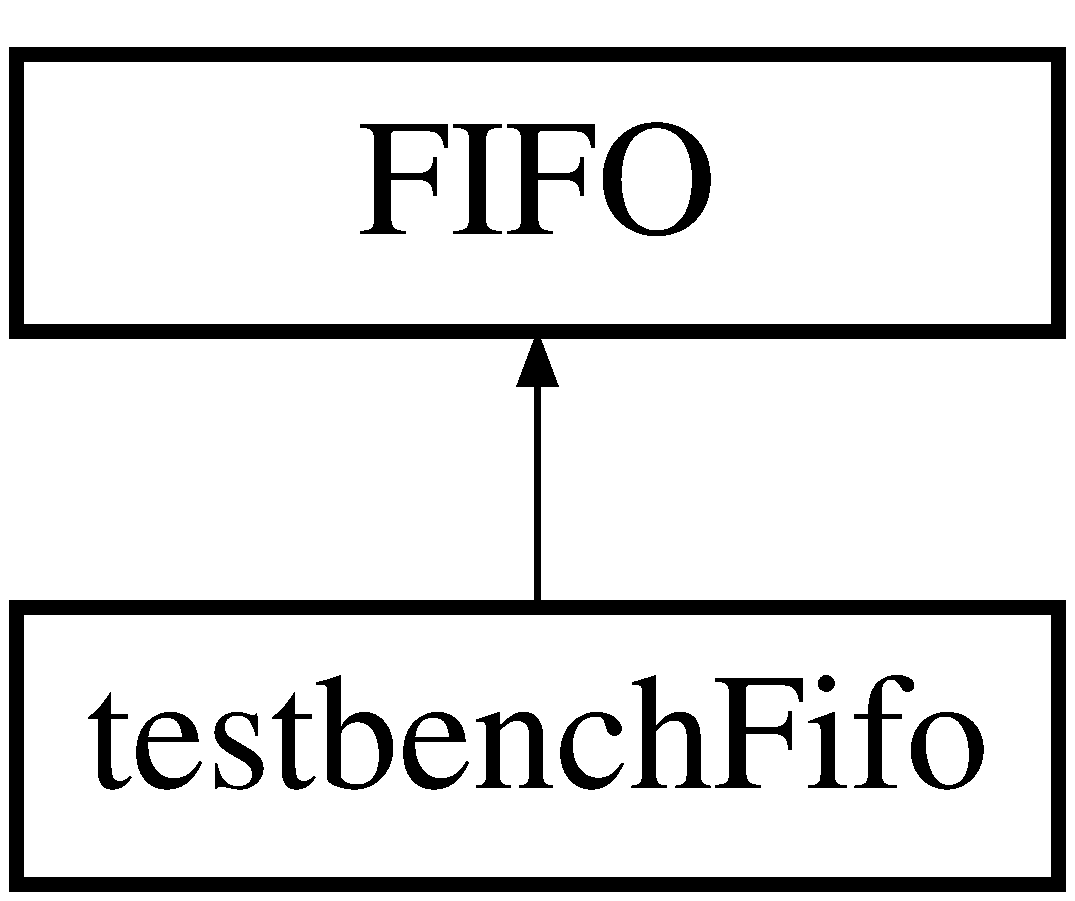
\includegraphics[height=2.000000cm]{classtestbenchFifo}
\end{center}
\end{figure}
\subsection*{Entities}
\begin{DoxyCompactItemize}
\item 
\hyperlink{classtestbenchFifo_1_1behavioural}{behavioural} architecture
\end{DoxyCompactItemize}
\subsection*{Libraries}
 \begin{DoxyCompactItemize}
\item 
\mbox{\Hypertarget{classtestbenchFifo_a0a6af6eef40212dbaf130d57ce711256}\label{classtestbenchFifo_a0a6af6eef40212dbaf130d57ce711256}} 
\hyperlink{classtestbenchFifo_a0a6af6eef40212dbaf130d57ce711256}{ieee} 
\end{DoxyCompactItemize}
\subsection*{Use Clauses}
 \begin{DoxyCompactItemize}
\item 
\mbox{\Hypertarget{classtestbenchFifo_acd03516902501cd1c7296a98e22c6fcb}\label{classtestbenchFifo_acd03516902501cd1c7296a98e22c6fcb}} 
\hyperlink{classtestbenchFifo_acd03516902501cd1c7296a98e22c6fcb}{std\+\_\+logic\+\_\+1164}   
\end{DoxyCompactItemize}


The documentation for this class was generated from the following file\+:\begin{DoxyCompactItemize}
\item 
testbench\+Fifo.\+vhdl\end{DoxyCompactItemize}

\hypertarget{classtestbenchLcd}{}\section{testbench\+Lcd Entity Reference}
\label{classtestbenchLcd}\index{testbench\+Lcd@{testbench\+Lcd}}
Inheritance diagram for testbench\+Lcd\+:\begin{figure}[H]
\begin{center}
\leavevmode
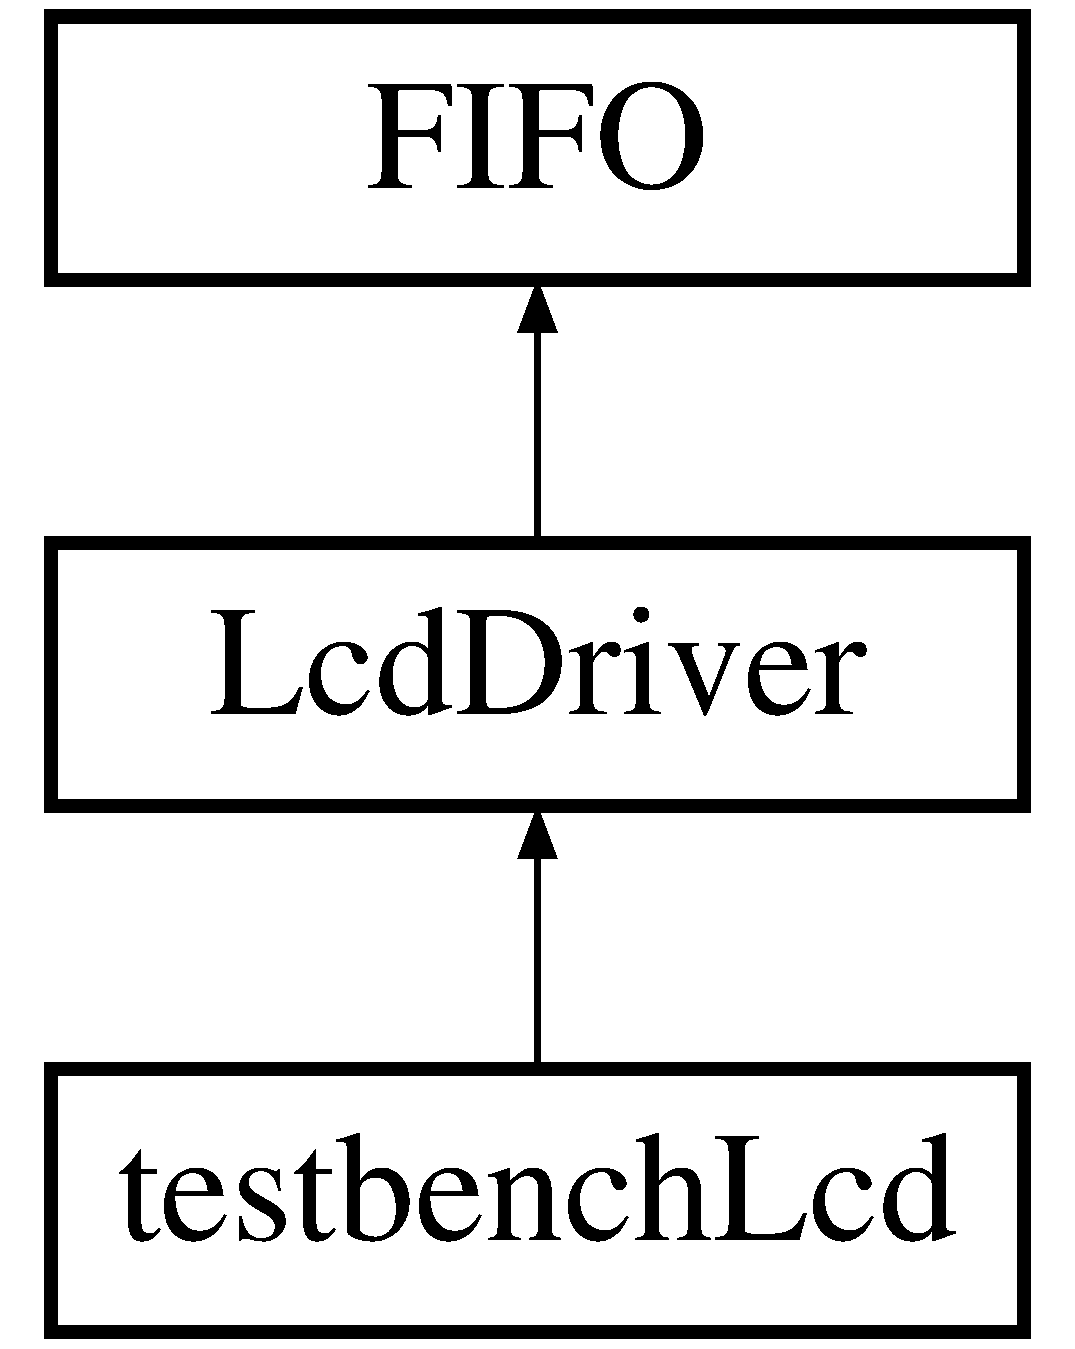
\includegraphics[height=3.000000cm]{classtestbenchLcd}
\end{center}
\end{figure}
\subsection*{Entities}
\begin{DoxyCompactItemize}
\item 
\hyperlink{classtestbenchLcd_1_1behavioural}{behavioural} architecture
\end{DoxyCompactItemize}
\subsection*{Libraries}
 \begin{DoxyCompactItemize}
\item 
\mbox{\Hypertarget{classtestbenchLcd_a0a6af6eef40212dbaf130d57ce711256}\label{classtestbenchLcd_a0a6af6eef40212dbaf130d57ce711256}} 
\hyperlink{classtestbenchLcd_a0a6af6eef40212dbaf130d57ce711256}{ieee} 
\end{DoxyCompactItemize}
\subsection*{Use Clauses}
 \begin{DoxyCompactItemize}
\item 
\mbox{\Hypertarget{classtestbenchLcd_acd03516902501cd1c7296a98e22c6fcb}\label{classtestbenchLcd_acd03516902501cd1c7296a98e22c6fcb}} 
\hyperlink{classtestbenchLcd_acd03516902501cd1c7296a98e22c6fcb}{std\+\_\+logic\+\_\+1164}   
\end{DoxyCompactItemize}


The documentation for this class was generated from the following file\+:\begin{DoxyCompactItemize}
\item 
testbench\+Lcd.\+vhdl\end{DoxyCompactItemize}

\hypertarget{classwriter}{}\section{writer Entity Reference}
\label{classwriter}\index{writer@{writer}}
\subsection*{Entities}
\begin{DoxyCompactItemize}
\item 
\hyperlink{classwriter_1_1behavioural}{behavioural} architecture
\end{DoxyCompactItemize}
\subsection*{Libraries}
 \begin{DoxyCompactItemize}
\item 
\mbox{\Hypertarget{classwriter_a0a6af6eef40212dbaf130d57ce711256}\label{classwriter_a0a6af6eef40212dbaf130d57ce711256}} 
\hyperlink{classwriter_a0a6af6eef40212dbaf130d57ce711256}{ieee} 
\end{DoxyCompactItemize}
\subsection*{Use Clauses}
 \begin{DoxyCompactItemize}
\item 
\mbox{\Hypertarget{classwriter_acd03516902501cd1c7296a98e22c6fcb}\label{classwriter_acd03516902501cd1c7296a98e22c6fcb}} 
\hyperlink{classwriter_acd03516902501cd1c7296a98e22c6fcb}{std\+\_\+logic\+\_\+1164}   
\end{DoxyCompactItemize}
\subsection*{Ports}
 \begin{DoxyCompactItemize}
\item 
\mbox{\Hypertarget{classwriter_a868bf8dd825e7fe9c3b5451faf25fcdf}\label{classwriter_a868bf8dd825e7fe9c3b5451faf25fcdf}} 
\hyperlink{classwriter_a868bf8dd825e7fe9c3b5451faf25fcdf}{Clk\+\_\+\+CI}  {\bfseries {\bfseries \textcolor{vhdlchar}{in}\textcolor{vhdlchar}{ }}} {\bfseries \textcolor{vhdlchar}{std\+\_\+logic}\textcolor{vhdlchar}{ }} 
\item 
\mbox{\Hypertarget{classwriter_ac1c93d2f55fe023a5d3ad03aeb8afe6a}\label{classwriter_ac1c93d2f55fe023a5d3ad03aeb8afe6a}} 
\hyperlink{classwriter_ac1c93d2f55fe023a5d3ad03aeb8afe6a}{Address\+\_\+\+DI}  {\bfseries {\bfseries \textcolor{vhdlchar}{in}\textcolor{vhdlchar}{ }}} {\bfseries \textcolor{vhdlchar}{std\+\_\+logic\+\_\+vector}\textcolor{vhdlchar}{ }\textcolor{vhdlchar}{(}\textcolor{vhdlchar}{ }\textcolor{vhdlchar}{ } \textcolor{vhdldigit}{2} \textcolor{vhdlchar}{ }\textcolor{vhdlchar}{downto}\textcolor{vhdlchar}{ }\textcolor{vhdlchar}{ } \textcolor{vhdldigit}{0} \textcolor{vhdlchar}{ }\textcolor{vhdlchar}{)}\textcolor{vhdlchar}{ }} 
\item 
\mbox{\Hypertarget{classwriter_a159dd0ab062d7714a5e7e4478bcb201e}\label{classwriter_a159dd0ab062d7714a5e7e4478bcb201e}} 
\hyperlink{classwriter_a159dd0ab062d7714a5e7e4478bcb201e}{Write\+\_\+\+SI}  {\bfseries {\bfseries \textcolor{vhdlchar}{in}\textcolor{vhdlchar}{ }}} {\bfseries \textcolor{vhdlchar}{std\+\_\+logic}\textcolor{vhdlchar}{ }} 
\item 
\mbox{\Hypertarget{classwriter_a331ece18a5e52c4e8df57e5aa4182824}\label{classwriter_a331ece18a5e52c4e8df57e5aa4182824}} 
\hyperlink{classwriter_a331ece18a5e52c4e8df57e5aa4182824}{Write\+Data\+\_\+\+DI}  {\bfseries {\bfseries \textcolor{vhdlchar}{in}\textcolor{vhdlchar}{ }}} {\bfseries \textcolor{vhdlchar}{std\+\_\+logic\+\_\+vector}\textcolor{vhdlchar}{ }\textcolor{vhdlchar}{(}\textcolor{vhdlchar}{ }\textcolor{vhdlchar}{ } \textcolor{vhdldigit}{7} \textcolor{vhdlchar}{ }\textcolor{vhdlchar}{downto}\textcolor{vhdlchar}{ }\textcolor{vhdlchar}{ } \textcolor{vhdldigit}{0} \textcolor{vhdlchar}{ }\textcolor{vhdlchar}{)}\textcolor{vhdlchar}{ }} 
\item 
\mbox{\Hypertarget{classwriter_ab1a2ea9b1494787f952f9e50311c7005}\label{classwriter_ab1a2ea9b1494787f952f9e50311c7005}} 
\hyperlink{classwriter_ab1a2ea9b1494787f952f9e50311c7005}{Reg\+Dir\+\_\+\+DO}  {\bfseries {\bfseries \textcolor{vhdlchar}{out}\textcolor{vhdlchar}{ }}} {\bfseries \textcolor{vhdlchar}{std\+\_\+logic\+\_\+vector}\textcolor{vhdlchar}{ }\textcolor{vhdlchar}{(}\textcolor{vhdlchar}{ }\textcolor{vhdlchar}{ } \textcolor{vhdldigit}{7} \textcolor{vhdlchar}{ }\textcolor{vhdlchar}{downto}\textcolor{vhdlchar}{ }\textcolor{vhdlchar}{ } \textcolor{vhdldigit}{0} \textcolor{vhdlchar}{ }\textcolor{vhdlchar}{)}\textcolor{vhdlchar}{ }} 
\item 
\mbox{\Hypertarget{classwriter_a1f43ab6af4ed4997c825beeecb67c6f0}\label{classwriter_a1f43ab6af4ed4997c825beeecb67c6f0}} 
\hyperlink{classwriter_a1f43ab6af4ed4997c825beeecb67c6f0}{Reg\+Port\+\_\+\+D\+IO}  {\bfseries {\bfseries \textcolor{vhdlchar}{inout}\textcolor{vhdlchar}{ }}} {\bfseries \textcolor{vhdlchar}{std\+\_\+logic\+\_\+vector}\textcolor{vhdlchar}{ }\textcolor{vhdlchar}{(}\textcolor{vhdlchar}{ }\textcolor{vhdlchar}{ } \textcolor{vhdldigit}{7} \textcolor{vhdlchar}{ }\textcolor{vhdlchar}{downto}\textcolor{vhdlchar}{ }\textcolor{vhdlchar}{ } \textcolor{vhdldigit}{0} \textcolor{vhdlchar}{ }\textcolor{vhdlchar}{)}\textcolor{vhdlchar}{ }} 
\item 
\mbox{\Hypertarget{classwriter_a33c132776119892469f53f02d193b0e8}\label{classwriter_a33c132776119892469f53f02d193b0e8}} 
\hyperlink{classwriter_a33c132776119892469f53f02d193b0e8}{I\+R\+Q\+Ctrl\+\_\+\+SO}  {\bfseries {\bfseries \textcolor{vhdlchar}{out}\textcolor{vhdlchar}{ }}} {\bfseries \textcolor{vhdlchar}{std\+\_\+logic}\textcolor{vhdlchar}{ }} 
\item 
\mbox{\Hypertarget{classwriter_a088e58e610bbc1ffae13fde6efdf06dc}\label{classwriter_a088e58e610bbc1ffae13fde6efdf06dc}} 
\hyperlink{classwriter_a088e58e610bbc1ffae13fde6efdf06dc}{I\+R\+Q\+State\+\_\+\+SO}  {\bfseries {\bfseries \textcolor{vhdlchar}{out}\textcolor{vhdlchar}{ }}} {\bfseries \textcolor{vhdlchar}{std\+\_\+logic}\textcolor{vhdlchar}{ }} 
\end{DoxyCompactItemize}


The documentation for this class was generated from the following file\+:\begin{DoxyCompactItemize}
\item 
writer.\+vhdl\end{DoxyCompactItemize}

\chapter{File Documentation}
\hypertarget{lcdDriver_8vhdl}{}\section{lcd\+Driver.\+vhdl File Reference}
\label{lcdDriver_8vhdl}\index{lcd\+Driver.\+vhdl@{lcd\+Driver.\+vhdl}}


L\+CD driver. Translates avalon bus data and commands to the L\+CD interface.  


\subsection*{Entities}
\begin{DoxyCompactItemize}
\item 
\hyperlink{classLcdDriver}{Lcd\+Driver} entity
\item 
\hyperlink{classLcdDriver_1_1LCD}{L\+CD} architecture
\end{DoxyCompactItemize}


\subsection{Detailed Description}
L\+CD driver. Translates avalon bus data and commands to the L\+CD interface. 

\begin{DoxyAuthor}{Author}
David Wright 
\end{DoxyAuthor}

%--- End generated contents ---

% Index
\backmatter
\newpage
\phantomsection
\clearemptydoublepage
\addcontentsline{toc}{chapter}{Index}
\printindex

\end{document}
